\documentclass[tikz,10pt]{beamer}
\usepackage[utf8]{inputenc}
\usepackage[T1]{fontenc}
\usetheme{default}
\usepackage{lipsum}
\usepackage{listings}

% ----------------------------
% fabio - headers
% ----------------------------

\usepackage{tikz}
\usetikzlibrary{matrix,arrows.meta}

\begin{document}
	\author{Bruno Canale \\ Bruno Giordano \\ Fábio Sancinetti \\
		Wanderson Ferreira}
	\title{Estudos sobre Redes Neurais Convolucionais}
	\subtitle{Disciplina PSI5886 \\ Prof. Emilio Del
		Moral Hernandez}
	%\logo{}
	%\institute{}
	\date{\today}
	%\subject{}
	%\setbeamercovered{transparent}
	%\setbeamertemplate{navigation symbols}{}
	\maketitle
	\begin{frame}
		\frametitle{Objetivos do Trabalho}
		
		Os objetivos principais do trabalho foram:
		
		\begin{itemize}
			\item Entender como as \textbf{MLPs} clássicas evoluíram para o que hoje é conhecido como Deep Learning
			\item Estudar a estrutura e o funcionamento de Redes Neurais
			Convolucionais 2D
			\item Entender como a informação é transformada dentro da
			rede neural ao avançar nas camadas mais profundas
			\item Extrapolar esse conhecimento para redes mais
			clássicas como a \textbf{MLP} estudada durante a
			disciplina.
		\end{itemize}
	\end{frame}
	
	\begin{frame}
		\frametitle{Introdução e Motivação}
		\begin{itemize}
			\item Cybenko prova que uma rede neural MLP com uma camada escondida e com número arbitrário de neurônios consegue aproximar qualquer função
			
			\item Considerando tal resultado, por que tentar fazer redes neurais profundas?
			
			\item Delalleau e Bengio fizeram um estudo teórico \footnote{O. Delalleau, Y. Bengio - \emph{Shallow vs Deep Sum-Product Networks},
				\hskip 1em plus
				0.5em minus 0.4em\relax Neural Information Processing Systems} com neurônios simples (chamados de sum-product units) comparando a quantidade de neurônios necessária para uma aproximação com redes "superficiais" e "profundas"
			
			\item O trabalho conclui que para algumas classes de funções a utilização de redes neurais como postuladas por Cybenko requer um número de neurônios consideravelmente maior à uma rede neural com mais camadas escondidas
			
			\item Tarefas clássicas de inteligência artificial (como reconhecimento de imagens) se encaixam em algumas dessas premissas, justificando a utilização de arquiteturas profundas nesses problemas
			
			
		\end{itemize}
		
	\end{frame}
	
	\begin{frame}{Esboço da idéia do trabalho}
		
		\begin{itemize}
			\item \textbf{ Uma rede com $n$ inputs e profundidade $O(\log{n})$ pode representar com $O(n)$ units o que uma rede com profundidade 2 representaria com $O(2^{\sqrt{n}})$ units}
			\item Sejam \begin{cases}
				$N_1$ com 128 neurônios e profundidade 7 \\
				$N_2$ com $n$ neurônios e profundidade 2
			\end{cases}
			
			Temos $\sqrt{128} = 11.3 \Rightarrow 2^{11.3} = 2540$. Ou seja, $N_2$ necessitaria de quase 20 vezes mais neurônios para representar uma mesma função $f$.
		\end{itemize}
		
		
		\begin{figure}
			\centering
			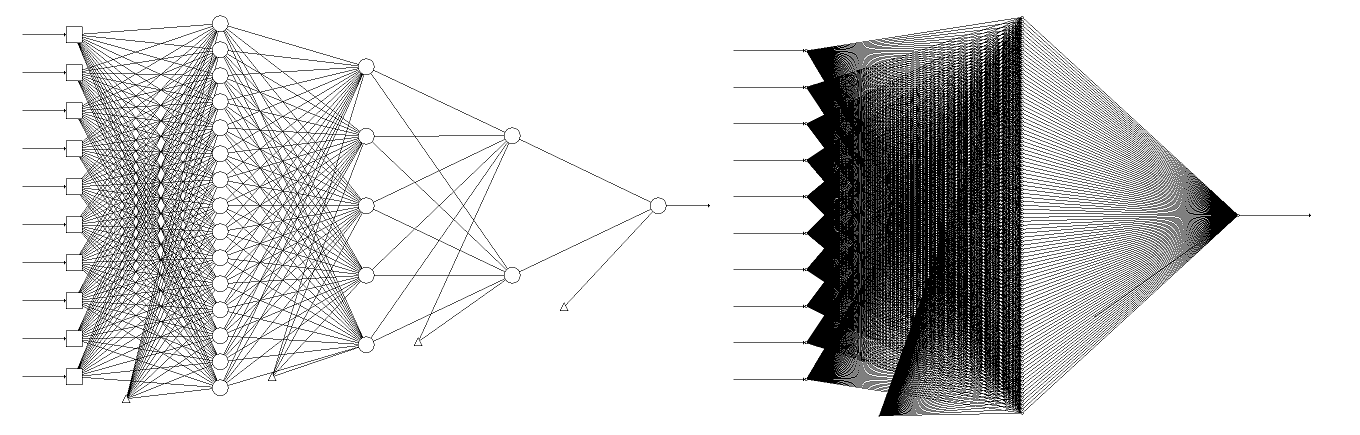
\includegraphics[scale=0.33]{images/shallowdeep.png}
		\end{figure}
		
		
	\end{frame}
	
	
	\begin{frame}
		\frametitle{Análise preliminar da MLP clássica vista em sala}
		
		Para entender os problemas no aprendizado de redes com grande número de camadas escondidas em uma MLP clássica, vamos relembrar alguns conceitos de rede neurais com a arquitetura profunda mais simples possível \footnote{Michael A. Nielsen. - \emph{Neural Networks and Deep Learning},
			\hskip 1em plus
			0.5em minus 0.4em\relax Determination Press, 2015} :
		
		
		\begin{figure}
			\centering
			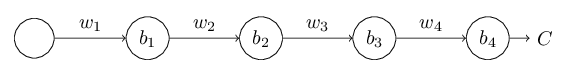
\includegraphics[scale=0.5]{nnetsimples.png}
		\end{figure}
		Seja $a_i$ o output do i-\'esimo neur\^onio do modelo. Ou seja:
		
		$$a = \begin{cases}
		a_1 = \sigma\big( w_1 x + b_1\big) = \sigma( z_1 ) \\
		a_i = \sigma\big( w_i a_{i-1} + b_i\big) = \sigma( z_i ) \enspace \enspace i>1
		\end{cases}$$
		
		Onde $\sigma(.)$ \'e a fun\c{c}\~ao de ativa\c{c}\~ao do i-\'esimo neur\^onio.
		A derivada parcial de $C$ em relação à $w_1$ pode ser calculada como:
		
		$$ \frac{\partial C}{\partial w_1} = x \cdot \sigma^{'}(z_1) \cdot w_2 \cdot \sigma^{'}(z_2) \cdot w_3 \cdot \sigma^{'}(z_3) \cdot w_4 \cdot  \sigma^{'}(z_4)\cdot\frac{\partial C}{\partial a_4}$$
		
	\end{frame}
	
	\begin{frame}
		\frametitle{Funções de Perda}
		
		\begin{itemize}
			\item Erro quadrático médio (RMS)
			$$C = \frac{(y - a_4)^2}{2} = \frac{(y - \sigma(z_4))^2}{2} = \frac{(y - \sigma(a_3 w_4 + b_4))^2}{2}$$
			$$\frac{ \partial C } {\partial w_4 } =  \frac{ \partial a_4 } {\partial w_4 } \frac{ \partial C } {\partial a_4 } = a_3 \cdot \sigma^{'}(z_4) \cdot (\sigma(z_4) - y_{ref})$$
		\end{itemize}
		
		\begin{figure}
			\centering
			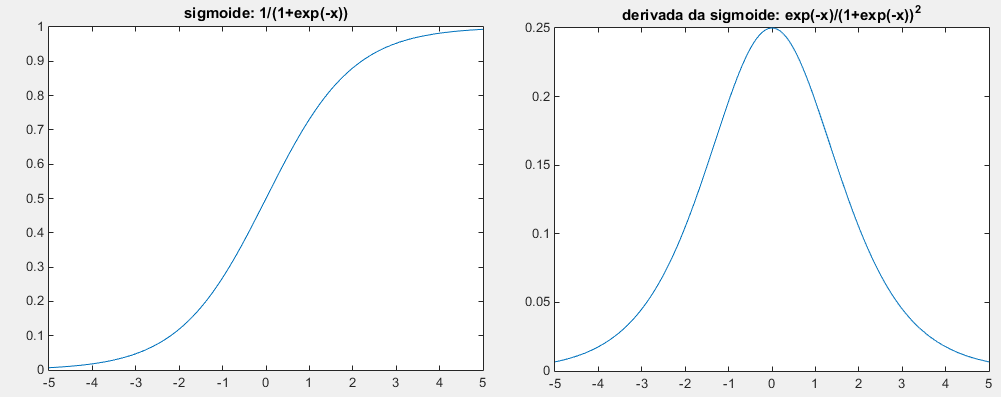
\includegraphics[scale=0.33]{images/plots.png}
		\end{figure}
		
		
		
	\end{frame}
	
	\begin{frame}
		\frametitle{Funções de Perda}
		
		\begin{itemize}
			\item Treino com RMS
		\end{itemize}
		\begin{figure}
			\centering
			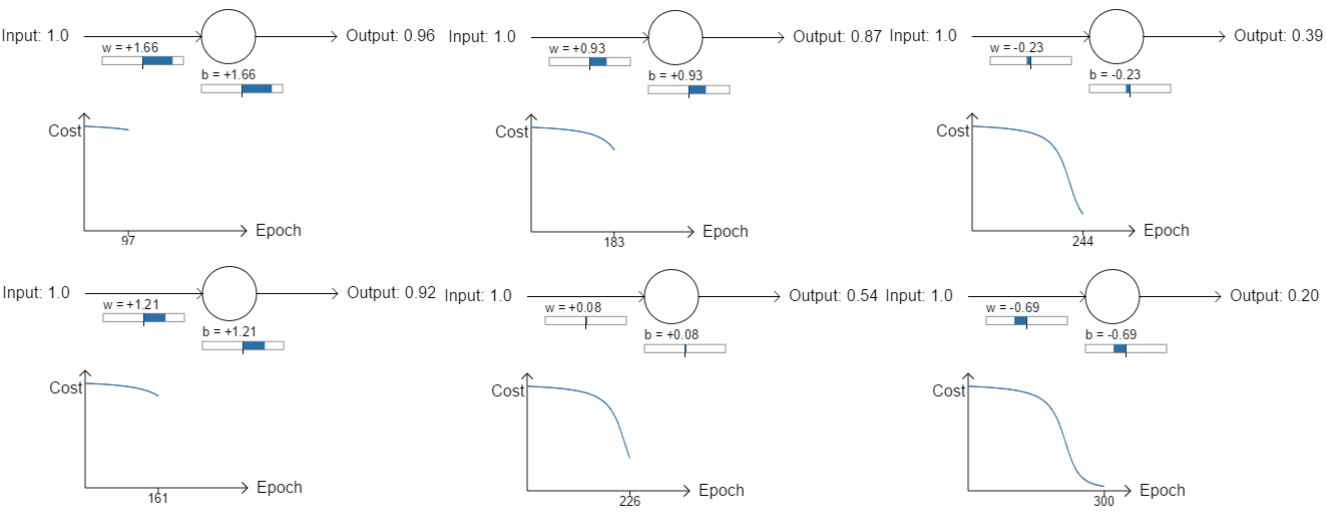
\includegraphics[scale=0.33]{images/training.png}
		\end{figure} Script disponivel em \footnote{Michael A. Nielsen. - \emph{Neural Networks and Deep Learning},
		\hskip 1em plus
		0.5em minus 0.4em\relax Determination Press, 2015
		http://neuralnetworksanddeeplearning.com/chap3.html}.
	
	
\end{frame}

\begin{frame}
	\frametitle{Funções de Perda}
	
	\begin{itemize}
		\item Cross-entropy loss:
		$$C = - \bigg(y_{ref} \ln{a_4} + (1-y_{ref}) \ln{(1 - a_4)} \bigg) \Rightarrow \Big(a_4 = \sigma(z_4) \Big) \Rightarrow $$
		$$\frac{ \partial C } {\partial w_4 } = a_3 \cdot \sigma^{'}(z_4) \cdot \bigg(- \frac{ y_{ref} }{ \sigma(z_4)} + \frac{(1 - y_{ref})}{1 -  \sigma(z_4)} \bigg) = $$ 
		$$ \frac{ \partial C } {\partial w_4 }  = a_3 \frac{ \sigma^{'}(z_4) } { \sigma(z_4)(1 -  \sigma(z_4)) }  \Big(\sigma(z_4) - y_{ref}\Big)$$
		
		Para a sigmoide $\sigma = \frac{1}{1 + e^{-z}}$, temos $\sigma^{'} = \sigma(1-\sigma)$. Assim:
		
		$$ \frac{ \partial C } {\partial w_4 }  = a_3 \frac{ \sigma(z_4)(1 -  \sigma(z_4))   } { \sigma(z_4)(1 -  \sigma(z_4)) }  \Big(\sigma(z_4) - y_{ref}\Big) = a_3 \Big(\sigma(z_4) - y_{ref}\Big) $$
		
		\item A derivada parcial $\frac{ \partial C } {\partial a_4 }$ "cancela" o termo $\sigma^{'}(z_4)$.
		\item Conceito pode ser estendido para outras funções de ativação.
		
	\end{itemize}
	
\end{frame}


\begin{frame}
	\frametitle{Funções de Perda}
	
	\begin{itemize}
		\item Treino com Cross-Entropy
	\end{itemize}
	\begin{figure}
		\centering
		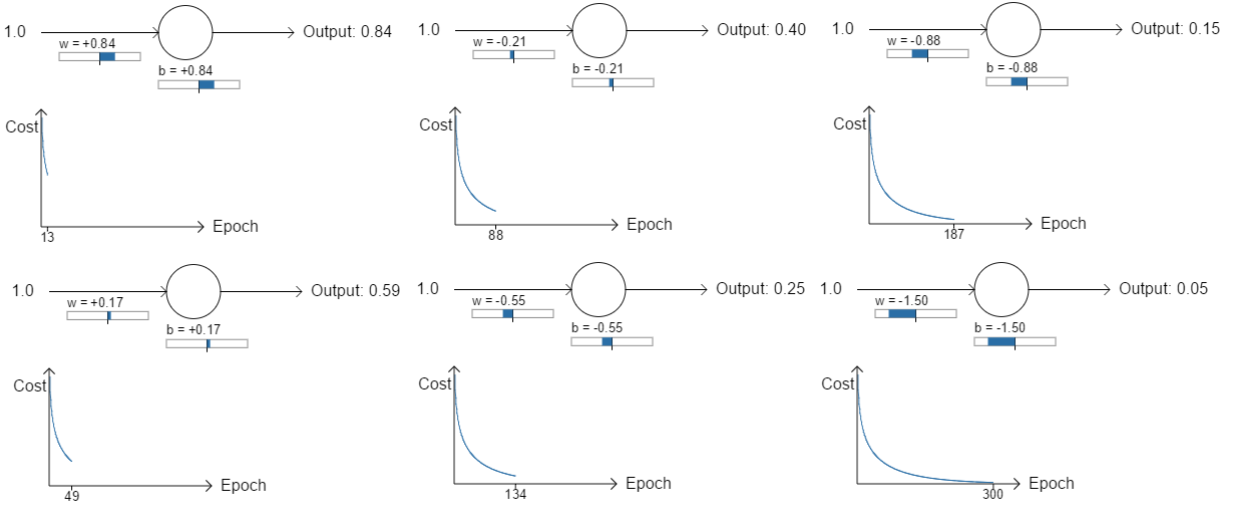
\includegraphics[scale=0.33]{images/trainingCE.png}
	\end{figure} Script disponivel em \footnote{Michael A. Nielsen. - \emph{Neural Networks and Deep Learning},
	\hskip 1em plus
	0.5em minus 0.4em\relax Determination Press, 2015 http://neuralnetworksanddeeplearning.com/chap3.html}.


\end{frame}

\begin{frame}
	\frametitle{Problema Vanishing Gradient}
	Vamos voltar a analisar $\frac{\partial C}{\partial w_1}$:
	
	$$ \frac{\partial C}{\partial w_1} = x \cdot \sigma^{'}(z_1) \cdot w_2 \cdot \sigma^{'}(z_2) \cdot w_3 \cdot \sigma^{'}(z_3) \cdot w_4 \cdot  \sigma^{'}(z_4)\cdot\frac{\partial C}{\partial a_4} \rightarrow $$
	\begin{figure}
		\centering
		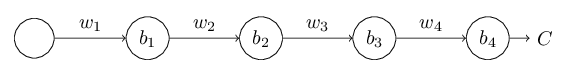
\includegraphics[scale=0.5]{nnetsimples.png}
	\end{figure}
	$$ \frac{\partial C}{\partial w_1} = x \bigg(w_2 w_3 w_4 \bigg) \cdot \bigg(\sigma^{'}(z_1) \cdot \sigma^{'}(z_2)\cdot \sigma^{'}(z_3) \cdot \sigma^{'}(z_4) \bigg) \frac{\partial C}{\partial a_4} $$
	
	\begin{itemize}
		\item Como $\sigma^{'}(z) \leq 0.25$, a multiplicação de vários $\sigma^{'}(z)$ resulta em valores cada vez menores.
		
		\item Quanto maior a "distância" entre a camada e a função de perda $C$, menor a velocidade de aprendizado.
		
		\item Se inicializarmos todos os pesos com a mesma distribuição aleatória sem considerar a profundidade da camada em que se encontram, teremos uma inicialização com $\frac{\partial C}{\partial w_1} < \frac{\partial C}{\partial w_2} < \frac{\partial C}{\partial w_3} < ... $
	\end{itemize}
	
\end{frame}

\begin{frame}
	\frametitle{Problema Vanishing Gradient}
	
	\begin{itemize}
		\item Rede com 4 camadas escondidas com o mesmo número de neurônios, treinada no dataset MNIST (banco de dados de números escritos à mão)
		\item Para cada iteração do treino, a norma das alterações $\Delta w_i$ dos pesos é usada para inferir a velocidade de aprendizado
	\end{itemize}
	
	\begin{figure}
		\centering
		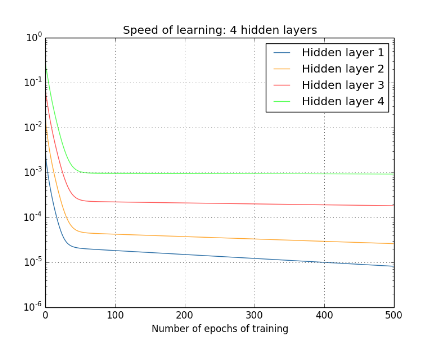
\includegraphics[scale=0.6]{images/vanishinggradient.png}
	\end{figure}
	Imagem disponível em \footnote{Michael A. Nielsen. - \emph{Neural Networks and Deep Learning},
		\hskip 1em plus
		0.5em minus 0.4em\relax Determination Press, 2015 http://neuralnetworksanddeeplearning.com/chap5.html}.
	
\end{frame}

\begin{frame}
	\frametitle{Deep Learning}
	\begin{itemize}
		\item Diversos outros problemas associados a escalabilidade de redes neurais
		\item Estudo de técnicas para possibilitar treinamento de arquiteturas profundas
		\item Hyper-parâmetros para serem selecionados durante o treino, adequando-o conforme as especifidades dos dados
	\end{itemize}
\end{frame}

\begin{frame}
	\frametitle{Regularização}
	
	\begin{itemize}
		\item Consiste na inclusão de um termo extra na função de custo:
		$$C = C_{loss} + C_{reg}$$
		
		\item Esse termo $C_{reg}$ é usado para penalizar convergências indesejáveis durante o treino, introduzindo novos hyper-parametros
		
		\item Regularização L2:	    
		$$C^{L2}_{reg} = \lambda ||w||^2$$
		
		Penaliza otimizações com pesos $w$ altos. Conforme o aumento de $\lambda$, as sigmóides tendem a se ativar mais em torno da região linear:
		\begin{figure}
			\centering
			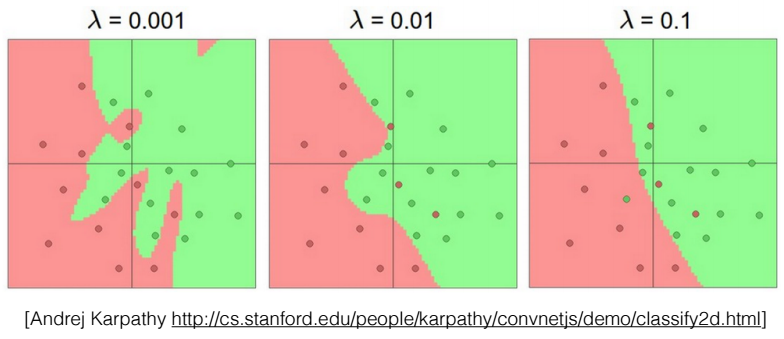
\includegraphics[scale=0.4]{images/regL2.png}
		\end{figure}
		
		
		
		
	\end{itemize}
	
	
\end{frame}


\begin{frame}
	\frametitle{Dropout}
	
	\begin{itemize}
		\item Técnica para evitar co-adaptação de neurônios
		\item Em cada iteração de treino, há uma probabilidade $p$ para cada neurônio estar ativo (pesos $w$ mantidos) e (1-p) de estar inativo (pesos $w$ zerados)
	\end{itemize}
	
	\begin{figure}
		\centering
		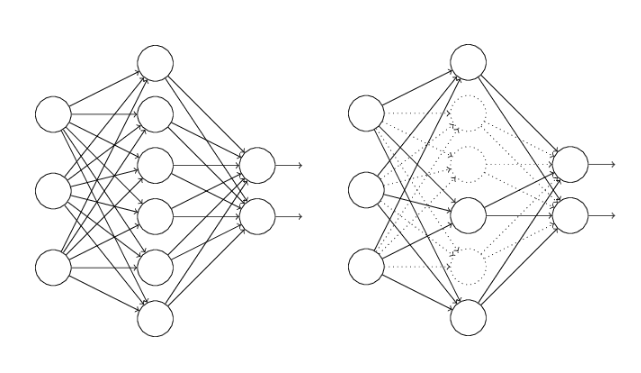
\includegraphics[scale=0.28]{dropout.png}
	\end{figure}
	
	
	\begin{itemize}
		\item Reduz a co-adaptação de neurônios
		\item Força os neurônios a aprenderem pesos baseados em diferentes subsets aleatórios de outros neurônios
		\item Melhora a capacidade de generalização para situações de oclusão de características
	\end{itemize}
	
\end{frame}


\begin{frame}
	\frametitle{Generalização de arquiteturas de ativação: building blocks}
	
	
	\begin{figure}
		\centering
		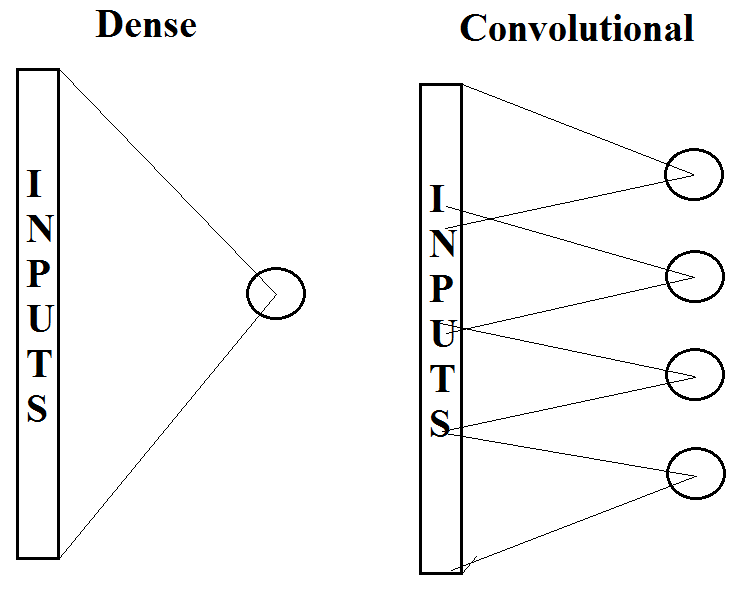
\includegraphics[scale=0.28]{images/denseconv.png}
	\end{figure}
	\begin{figure}
		\centering
		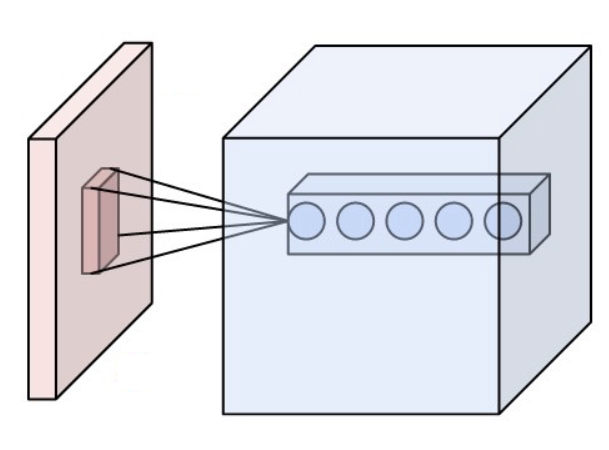
\includegraphics[scale=0.28]{images/conv.png}
	\end{figure}
	
\end{frame}



\begin{frame}
	\frametitle{Visualizando a Convolução}
	\centering
	\par \url{http://setosa.io/ev/image-kernels/}
	\par Explicação visual sobre Convoluções com demonstrações em Javascript
\end{frame}



\begin{frame}
	\frametitle{Visualizando a Convolução}
	\centering
\begin{figure}
	\centering
	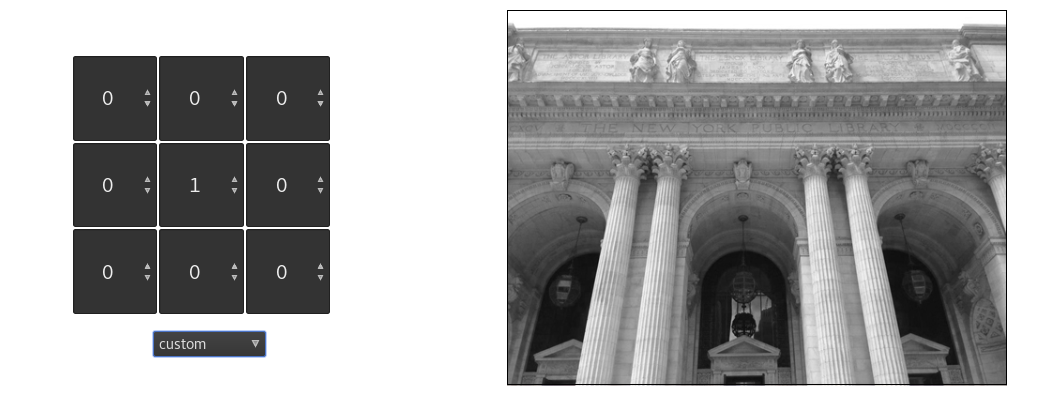
\includegraphics[width=1.0\linewidth]{images/convolucao/001_sem_filtro}
	\caption{Imagem original}
	\label{fig:001semfiltro}
\end{figure}

\end{frame}

\begin{frame}
	\frametitle{Visualizando a Convolução}
	\centering
\begin{figure}[t!]
	\centering
	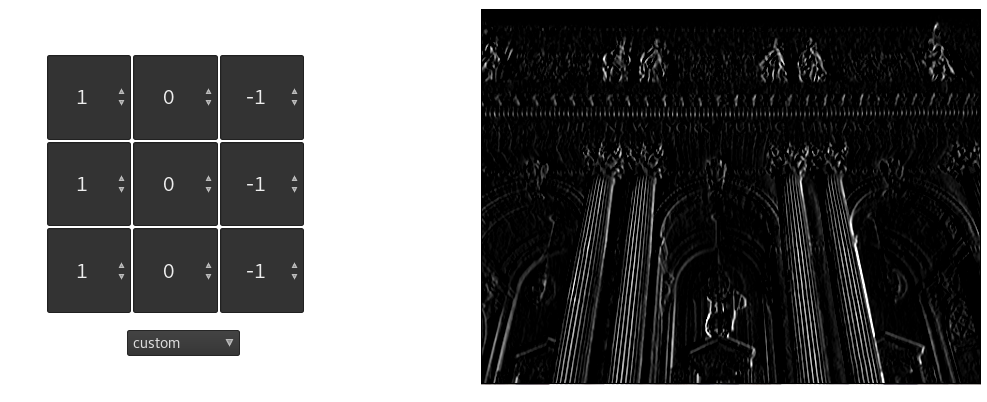
\includegraphics[width=0.7\linewidth]{images/convolucao/004_left_sobel} \\
	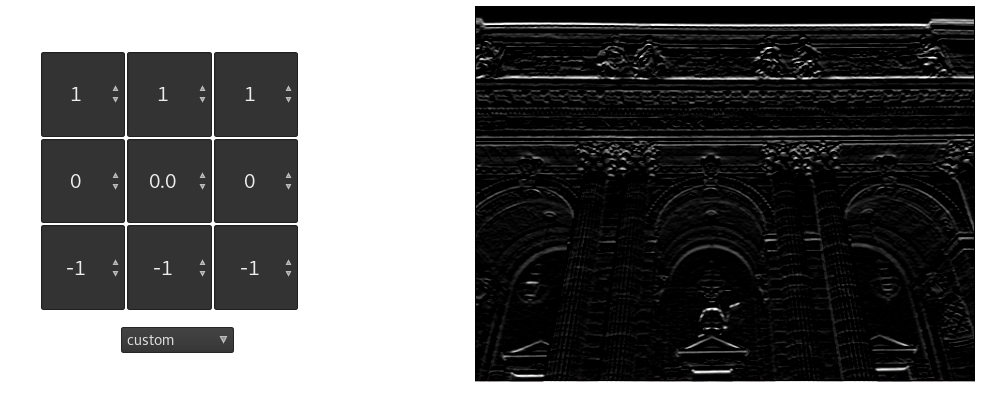
\includegraphics[width=0.7\linewidth]{images/convolucao/003_upper_sobel} \\
	\caption{Acima: efeito de \textit{Left Sobel}, Abaixo: Efeito \textit{Upper Sobel}}
	\label{fig:left_upper}
\end{figure}
\end{frame}


\begin{frame}
	\frametitle{Visualizando a Convolução}
	\centering
	
	\begin{figure}[t!]
		\centering
		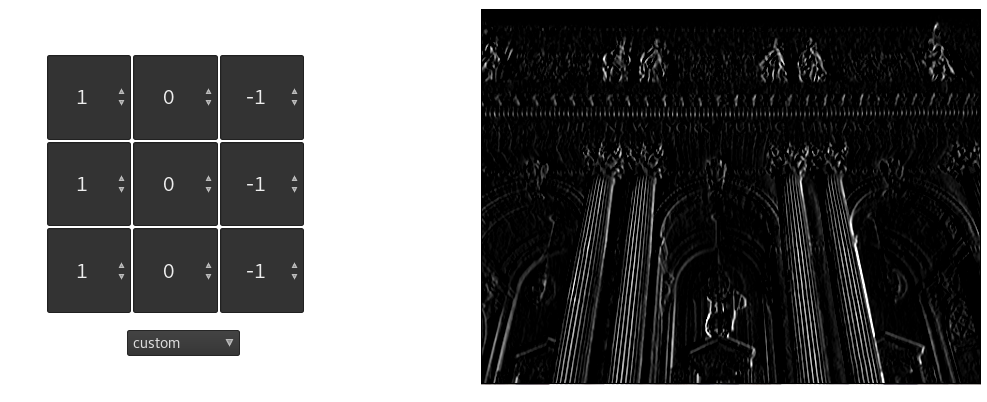
\includegraphics[width=0.7\linewidth]{images/convolucao/004_left_sobel} \\
		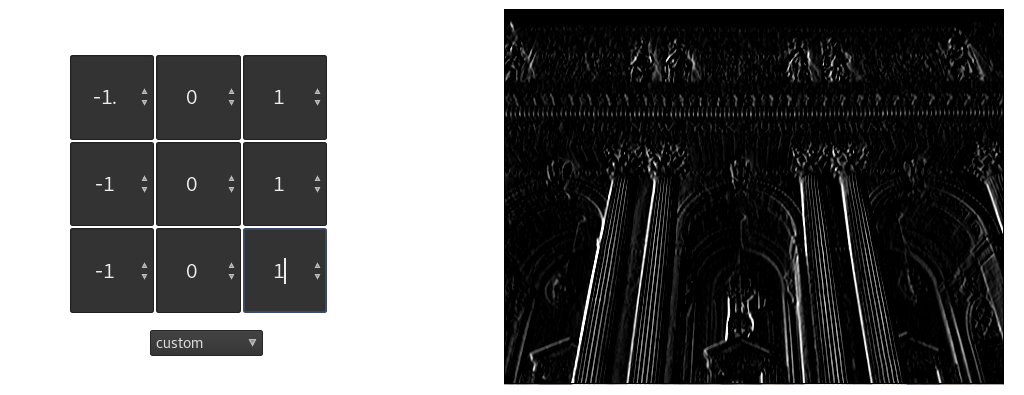
\includegraphics[width=0.7\linewidth]{images/convolucao/005_right_sobel} \\
		\caption{Acima: efeito de \textit{Left Sobel}, Abaixo: Efeito \textit{Right Sobel}}
		\label{fig:left_right_sobel}
	\end{figure}
\end{frame}

\begin{frame}
	\frametitle{Visualizando a Convolução}
	\centering
	\begin{figure}
		\centering
		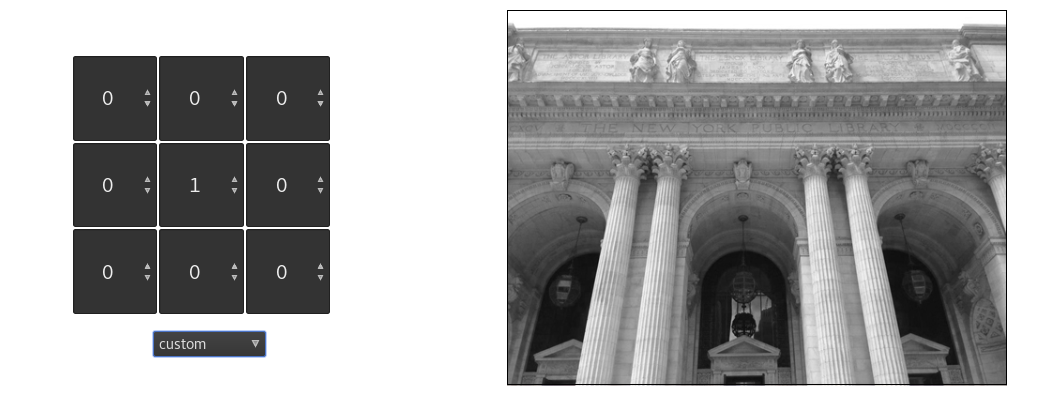
\includegraphics[width=0.7\linewidth]{images/convolucao/001_sem_filtro} \\
		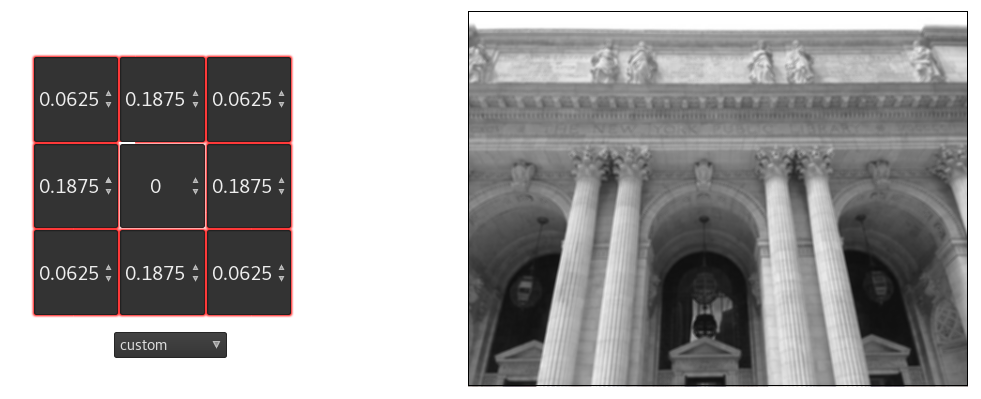
\includegraphics[width=0.7\linewidth]{images/convolucao/002_blur}		
		\caption{Acima: Imagem Original, Abaixo: Efeito \textit{Blur}}
		\label{fig:orig_blur}
	\end{figure}
	
\end{frame}


\begin{frame}
	\frametitle{Visualizando a Convolução}
	\centering
	\begin{figure}
		\centering
		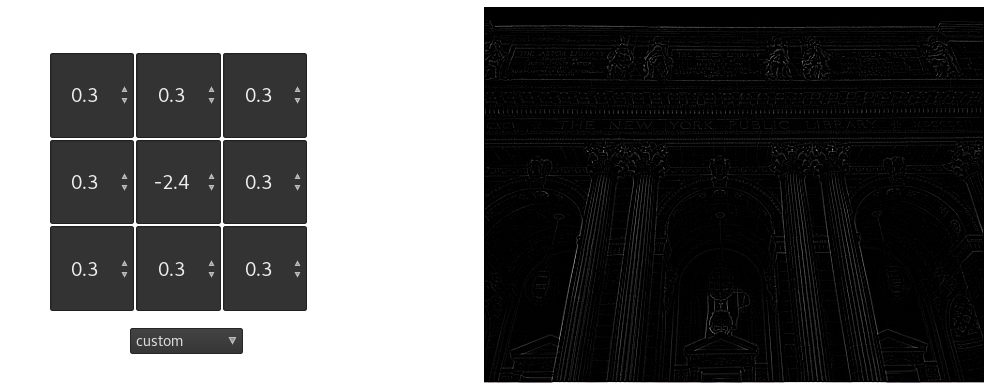
\includegraphics[width=1.0\linewidth]{images/convolucao/006_edge_det}		
		\caption{Exemplo trivial de detecção de bordas com filtro convolucional}
		\label{fig:orig_blur}
	\end{figure}
	
\end{frame}


\begin{frame}
	\frametitle{Base de dados utilizada - MNIST}
	
	\begin{columns}
		\begin{column}{0.48\textwidth}
			A base de dados MNIST é composta por 60.000 exemplos de
			imagens de digitos em letra cursivas. O dataset é ideal para
			testes de algoritmos em reconhecimentos de padrões por
			necessitar pouco pré-processamento.\\
			Mais informações no link: http://yann.lecun.com/exdb/mnist/
		\end{column}
		\begin{column}{0.48\textwidth}
			\begin{figure}
				\centering
				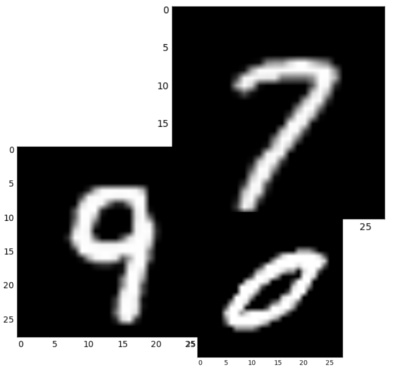
\includegraphics[scale=0.35]{minst}
			\end{figure}
		\end{column}
	\end{columns}
	
	\lstinputlisting[language=Python, firstline=0, lastline=10,
	basicstyle=\ttfamily\scriptsize]{base_import.py}
\end{frame}

  

\begin{frame}
	\frametitle{Processamento necessário no atributo target}
	
	Um processamento padrão é transformar o conjunto de
	\textbf{atributos targets} em um conjunto de variáveis
	categóricas. O que seriam variáveis categoricas?
	
	Exemplo: Se a lista de targets é composta por: [1.2, 2, 3, 4.2,
	4i] e as classes disponiveis são \textbf{real, inteiro,
		imaginario}, então uma matriz de transformação seria:
	
	\begin{table}[h]
		\caption{Conversão para variáveis categoricas}
		\begin{tabular}{l|c|c|c|}
			
			target & real & inteiro & imaginario \\
			1.2    & 1    & 0       & 0 \\
			2      & 0    & 1       & 0 \\
			3      & 0    & 1       & 0 \\
			4.2    & 1    & 0       & 0 \\
			4i     & 0    & 0       & 1
			
		\end{tabular}
	\end{table}
\end{frame}

\begin{frame}
	\frametitle{Implementação da Rede Convolucional 2D}
	\lstinputlisting[language=Python, firstline=0, lastline=25,
	basicstyle=\ttfamily\scriptsize]{cnn1.py}
\end{frame}

\begin{frame}
	\frametitle{Modelo do Experimento realizado para análise da
		Rede}
	\begin{itemize}
		\item Após implementação a arquitetura foi testada para
		verificar performance no conjunto de testes.
		\item Queriamos observar a transformação da imagem de Input
		após cada camada da ConvNet
		\item A fim de analisar com mais detalhes, foram adicionadas
		mais camadas convolucionais no modelo apresentado anteriormente.
	\end{itemize}
\end{frame}

% -------------------------------------------------
% \begin{fabio}
% -------------------------------------------------
\begin{frame}
	\frametitle{Entradas}
	\centering
	MNIST DATASET
	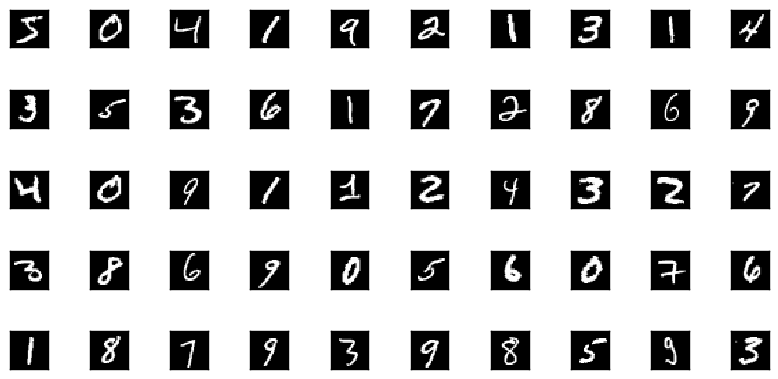
\includegraphics[width=.8\paperwidth]{images/fabio/inputs}
\end{frame}

\begin{frame}
	\frametitle{Exemplo de Rede}
	\centering
	
	\resizebox{!}{.9\textheight}{% if required
	\begin{tikzpicture}[
	start chain=going below,
	every join/.style={arrow},
	node distance=0.3cm
	]
	\node (start) [startstop,on chain,join] {Imagem de entrada};
	
	\node (out1) [process,on chain,join] {Convolução \\ Ativação};
	
	\node (out3) [process,on chain,join] {Convolução \\ Ativação };
	
	\node (out5) [process,on chain,join] {Convolução \\ Ativação};
	
	\node (out7) [process,on chain,join] {Pooling};

	\node (out8) [process,on chain,join] {Convolução \\ Ativação};
	
	\node (out10) [process,on chain,join] {Flatten};
	\node (out11) [process,on chain,join] {Dense};
	
	\node (out12) [process,on chain,join] {Dropout};
	\node (out13) [process,on chain,join] {Ativação};	
	
	\node (out14) [process,on chain,join] {Dense};
	\node (out15) [process,on chain,join] {Dropout};
			
	\node (out16) [startstop,on chain,join] {Ativação};		

	\end{tikzpicture}%
	}
\end{frame}


\begin{frame}
	\frametitle{Treinamento}
	\centering
%	\begin{minipage}{.5\textwidth}
		\centering
		\par Treinamento
		\begin{itemize}
			\item Épocas = 10
			\item Itens = 60.000
			\item Tempo = 30 $\longrightarrow$ 40 minutos
		\end{itemize}		
%	\end{minipage}%
%	\begin{minipage}{.5\textwidth}
	\centering
	\par Teste
	\begin{itemize}
		\item Itens = 10.000
	\end{itemize}	
\end{frame}

\begin{frame}
	\frametitle{Treinamento}		
	\centering
	\par Resultado na base de treinamento
	\begin{itemize}
		\item 98.94\%
	\end{itemize}	
	\begin{figure}
		\centering
		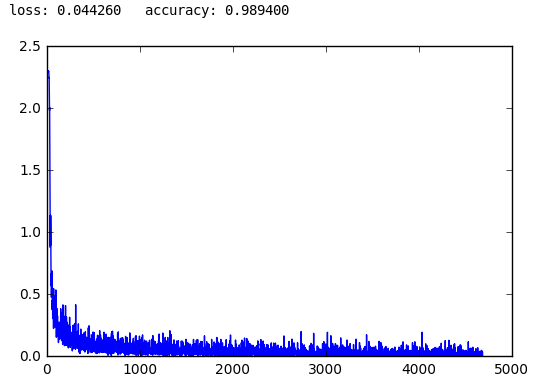
\includegraphics[width=0.5\linewidth]{images/resultados/network_1/loss_history}
		\label{fig:losshistory}
	\end{figure}
	\par Resultado na base de teste
	\begin{itemize}
		\item 99.06\%
	\end{itemize}	
%\end{minipage}%

\end{frame}

%%%%%%%%%%%%%%%%%%%%%%%%%%%%%%%%%%%%%%%%%%%%%%%%%%%%%%%%%%%%%%%%%%%%%%%%%%%%%%%%%%%%%%%%%%%
\begin{frame}
	\frametitle{Convolução - 1}
	\centering
	\begin{columns}
		\begin{column}{0.25\textwidth}
\begin{figure}
\resizebox{!}{.9\textheight}
{% if required
	
\begin{tikzpicture}[
start chain=going below,
every join/.style={arrow},
node distance=0.3cm
]
\node (start) [startstop,on chain,join] {Imagem de entrada};

\node (out1) [process2,on chain,join] {Convolução \\ Ativação};

\node (out3) [process,on chain,join] {Convolução \\ Ativação };

\node (out5) [process,on chain,join] {Convolução \\ Ativação};

\node (out7) [process,on chain,join] {Pooling};

\node (out8) [process,on chain,join] {Convolução \\ Ativação};

\node (out10) [process,on chain,join] {Flatten};
\node (out11) [process,on chain,join] {Dense};

\node (out12) [process,on chain,join] {Dropout};
\node (out13) [process,on chain,join] {Ativação};	

\node (out14) [process,on chain,join] {Dense};
\node (out15) [process,on chain,join] {Dropout};

\node (out16) [startstop,on chain,join] {Ativação};		

		\end{tikzpicture}
		} %resize		
			\end{figure}

		\end{column}		
	
		\begin{column}{0.25\textwidth}
			\begin{figure}
				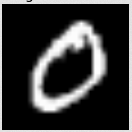
\includegraphics[height=.1\paperheight]{images/fabio/num_0}
				\caption{Entrada}
			\end{figure}%
		\end{column}
		\begin{column}{0.5\textwidth}
			\begin{figure}
			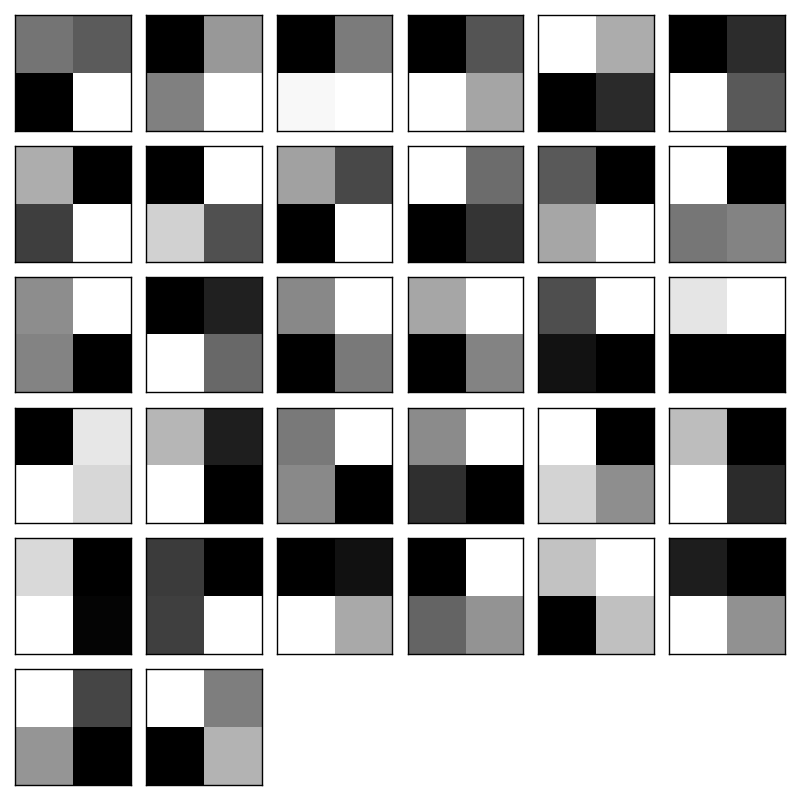
\includegraphics[height=.6\paperheight]{images/resultados/network_1/filter_convolution2d_1}%
			\caption{Filtros}			
			\end{figure}%
		\end{column}	
	\end{columns}

%	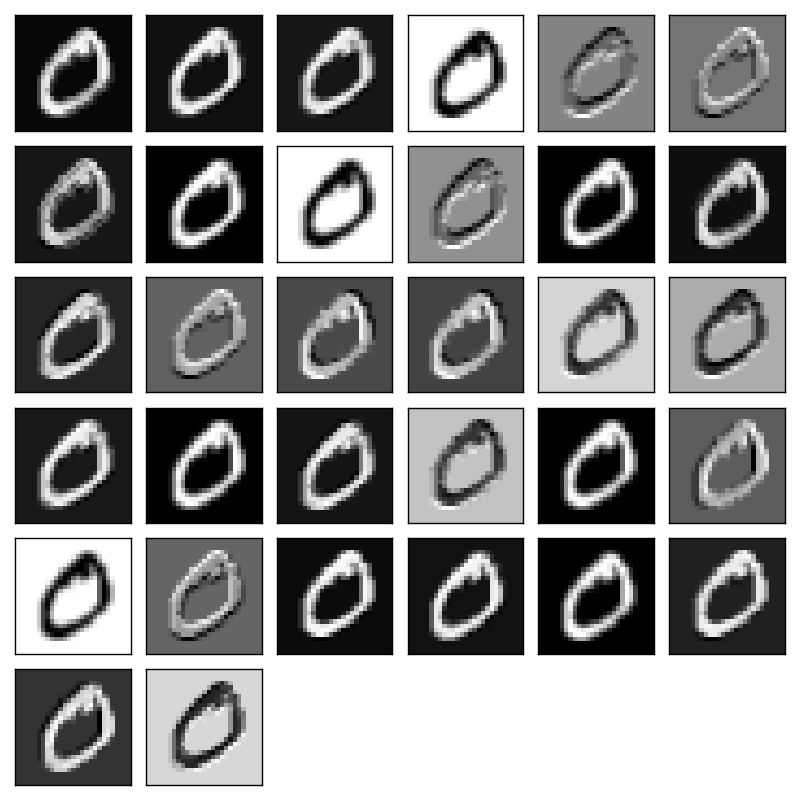
\includegraphics[height=.5\paperheight]{images/resultados/network_1/input_1_layer_convolution2d_1}		
\end{frame}
%%%%%%%%%%%%%%%%%%%%%%%%%%%%%%%%%%%%%%%%%%%%%%%%%%%%%%%%%%%%%%%%%%%%%%%%%%%%%%%%%%%%%%%%%%%

%%%%%%%%%%%%%%%%%%%%%%%%%%%%%%%%%%%%%%%%%%%%%%%%%%%%%%%%%%%%%%%%%%%%%%%%%%%%%%%%%%%%%%%%%%%
\begin{frame}
	\frametitle{Convolução - 1}
	\centering
	\begin{columns}
		\begin{column}{0.25\textwidth}
			\begin{figure}
				\resizebox{!}{.9\textheight}
				{% if required
					
					\begin{tikzpicture}[
					start chain=going below,
					every join/.style={arrow},
					node distance=0.3cm
					]
					\node (start) [startstop,on chain,join] {Imagem de entrada};
					
					\node (out1) [process2,on chain,join] {Convolução \\ Ativação};
					
					\node (out3) [process,on chain,join] {Convolução \\ Ativação };
					
					\node (out5) [process,on chain,join] {Convolução \\ Ativação};
					
					\node (out7) [process,on chain,join] {Pooling};
					
					\node (out8) [process,on chain,join] {Convolução \\ Ativação};
					
					\node (out10) [process,on chain,join] {Flatten};
					\node (out11) [process,on chain,join] {Dense};
					
					\node (out12) [process,on chain,join] {Dropout};
					\node (out13) [process,on chain,join] {Ativação};	
					
					\node (out14) [process,on chain,join] {Dense};
					\node (out15) [process,on chain,join] {Dropout};
					
					\node (out16) [startstop,on chain,join] {Ativação};		
					
					\end{tikzpicture}
				} %resize		
			\end{figure}
			
		\end{column}		
		
		\begin{column}{0.33\textwidth}
			\begin{figure}
				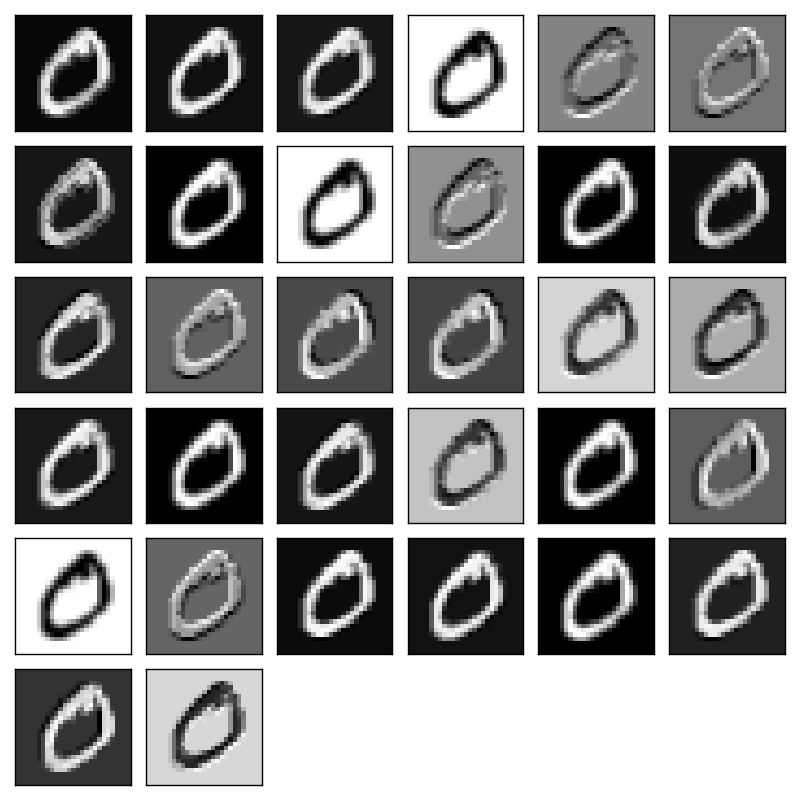
\includegraphics[height=4cm]{images/resultados/network_1/input_1_layer_convolution2d_1}
				\caption{Convolução 1}
			\end{figure}%
		\end{column}
		\begin{column}{0.33\textwidth}
			\begin{figure}
				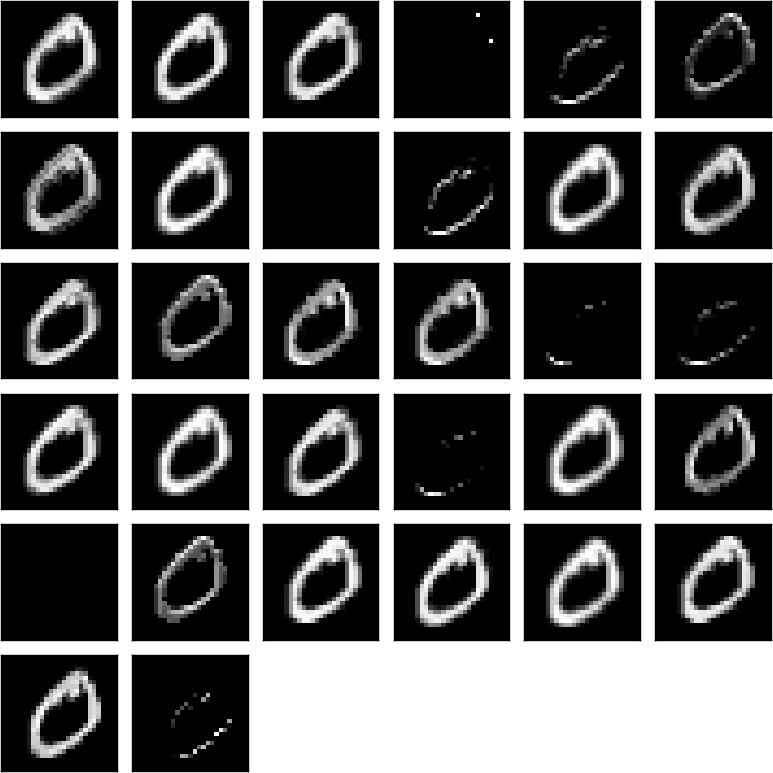
\includegraphics[height=4cm]{images/resultados/network_1/input_1_layer_activation_1}%
				\caption{Ativação}			
			\end{figure}%
		\end{column}	
	\end{columns}
	
\end{frame}
%%%%%%%%%%%%%%%%%%%%%%%%%%%%%%%%%%%%%%%%%%%%%%%%%%%%%%%%%%%%%%%%%%%%%%%%%%%%%%%%%%%%%%%%%%%

%%%%%%%%%%%%%%%%%%%%%%%%%%%%%%%%%%%%%%%%%%%%%%%%%%%%%%%%%%%%%%%%%%%%%%%%%%%%%%%%%%%%%%%%%%%
\begin{frame}
	\frametitle{Convolução - 2}
	\centering
	\begin{columns}
		\begin{column}{0.25\textwidth}
			\begin{figure}
				\resizebox{!}{.9\textheight}
				{% if required
					
					\begin{tikzpicture}[
					start chain=going below,
					every join/.style={arrow},
					node distance=0.3cm
					]
					\node (start) [startstop,on chain,join] {Imagem de entrada};
					
					\node (out1) [process3,on chain,join] {Convolução \\ Ativação};
					
					\node (out3) [process2,on chain,join] {Convolução \\ Ativação };
					
					\node (out5) [process,on chain,join] {Convolução \\ Ativação};
					
					\node (out7) [process,on chain,join] {Pooling};
					
					\node (out8) [process,on chain,join] {Convolução \\ Ativação};
					
					\node (out10) [process,on chain,join] {Flatten};
					\node (out11) [process,on chain,join] {Dense};
					
					\node (out12) [process,on chain,join] {Dropout};
					\node (out13) [process,on chain,join] {Ativação};	
					
					\node (out14) [process,on chain,join] {Dense};
					\node (out15) [process,on chain,join] {Dropout};
					
					\node (out16) [startstop,on chain,join] {Ativação};		
					
					\end{tikzpicture}
				} %resize		
			\end{figure}
			
		\end{column}		
		
		\begin{column}{0.33\textwidth}
			\begin{figure}
				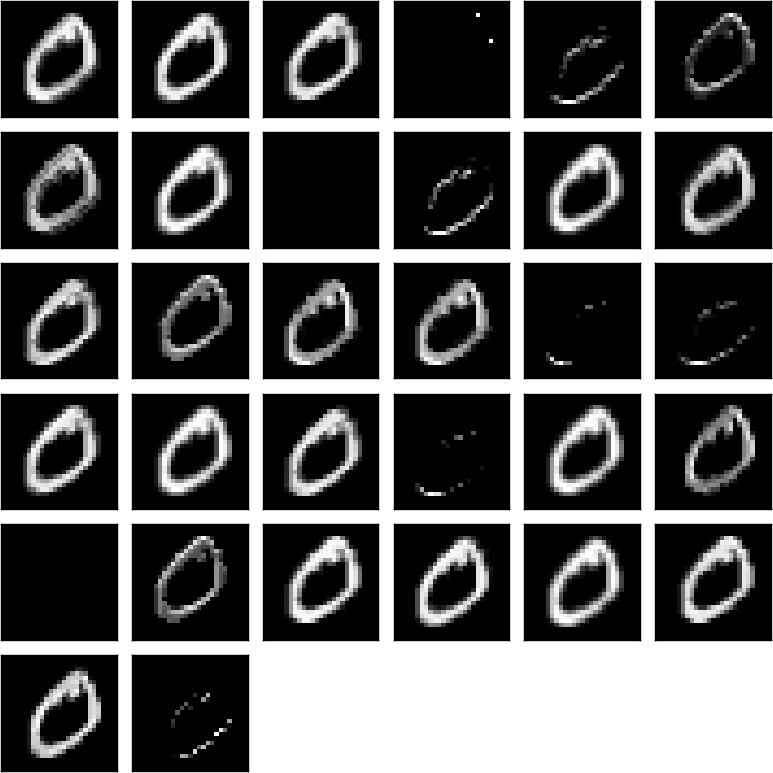
\includegraphics[height=4cm]{images/resultados/network_1/input_1_layer_activation_1}%
				\caption{Ativação 1}
			\end{figure}%
		\end{column}
		\begin{column}{0.33\textwidth}
			\begin{figure}
				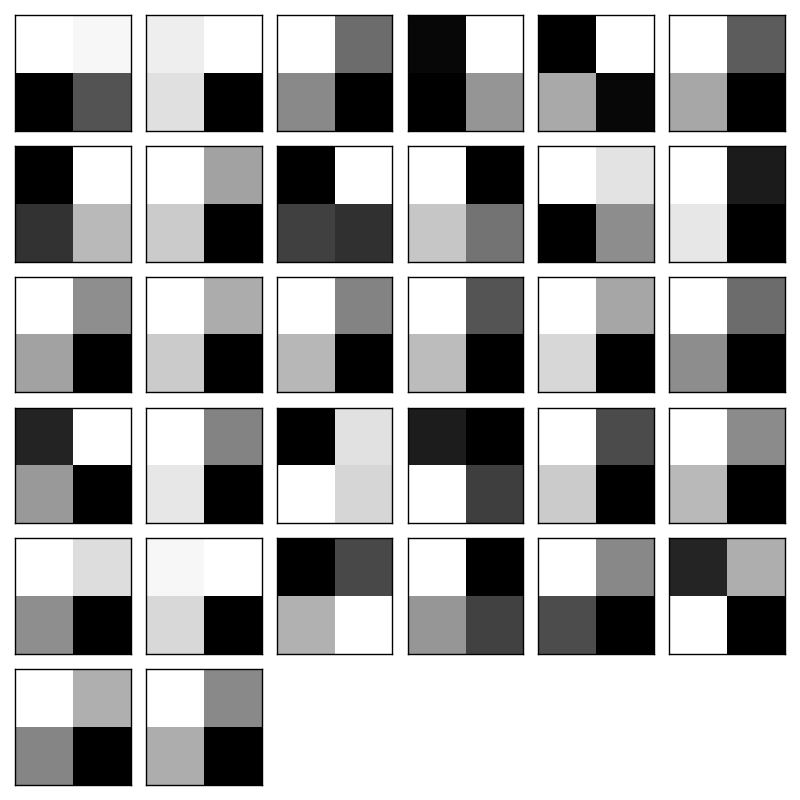
\includegraphics[height=4cm]{images/resultados/network_1/filter_convolution2d_2}%
				\caption{Filtros}			
			\end{figure}%
		\end{column}	
	\end{columns}
	
\end{frame}
%%%%%%%%%%%%%%%%%%%%%%%%%%%%%%%%%%%%%%%%%%%%%%%%%%%%%%%%%%%%%%%%%%%%%%%%%%%%%%%%%%%%%%%%%%%

%%%%%%%%%%%%%%%%%%%%%%%%%%%%%%%%%%%%%%%%%%%%%%%%%%%%%%%%%%%%%%%%%%%%%%%%%%%%%%%%%%%%%%%%%%%
\begin{frame}
	\frametitle{Convolução - 2}
	\centering
	\begin{columns}
		\begin{column}{0.25\textwidth}
			\begin{figure}
				\resizebox{!}{.9\textheight}
				{% if required
					
					\begin{tikzpicture}[
					start chain=going below,
					every join/.style={arrow},
					node distance=0.3cm
					]
					\node (start) [startstop,on chain,join] {Imagem de entrada};
					
					\node (out1) [process3,on chain,join] {Convolução \\ Ativação};
					
					\node (out3) [process2,on chain,join] {Convolução \\ Ativação };
					
					\node (out5) [process,on chain,join] {Convolução \\ Ativação};
					
					\node (out7) [process,on chain,join] {Pooling};
					
					\node (out8) [process,on chain,join] {Convolução \\ Ativação};
					
					\node (out10) [process,on chain,join] {Flatten};
					\node (out11) [process,on chain,join] {Dense};
					
					\node (out12) [process,on chain,join] {Dropout};
					\node (out13) [process,on chain,join] {Ativação};	
					
					\node (out14) [process,on chain,join] {Dense};
					\node (out15) [process,on chain,join] {Dropout};
					
					\node (out16) [startstop,on chain,join] {Ativação};		
					
					\end{tikzpicture}
				} %resize		
			\end{figure}
			
		\end{column}		
		
		\begin{column}{0.33\textwidth}
			\begin{figure}
				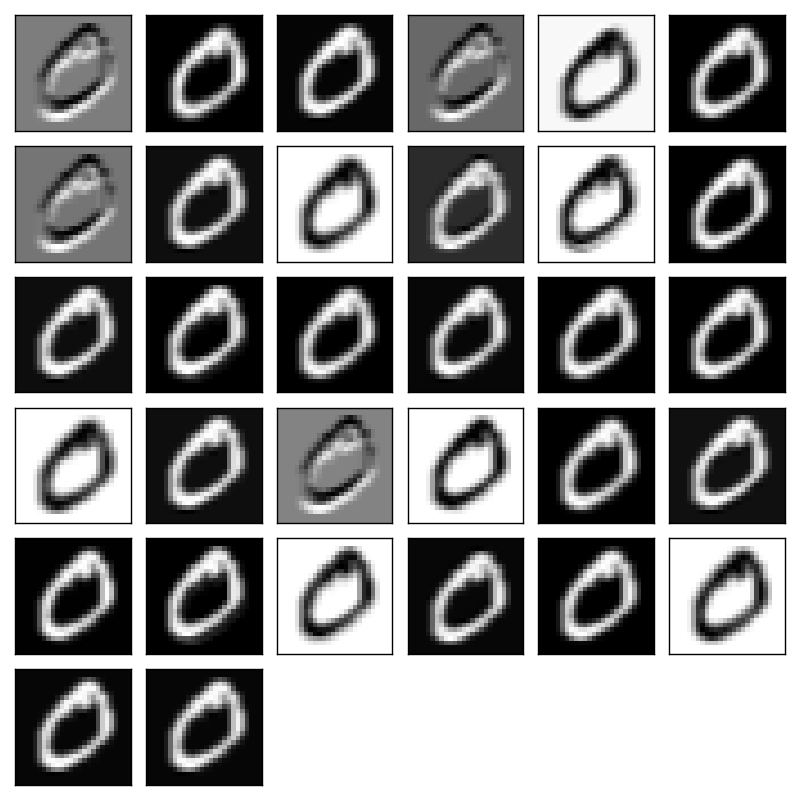
\includegraphics[height=4cm]{images/resultados/network_1/input_1_layer_convolution2d_2}%
				\caption{Convolução 2}
			\end{figure}%
		\end{column}
		\begin{column}{0.33\textwidth}
			\begin{figure}
				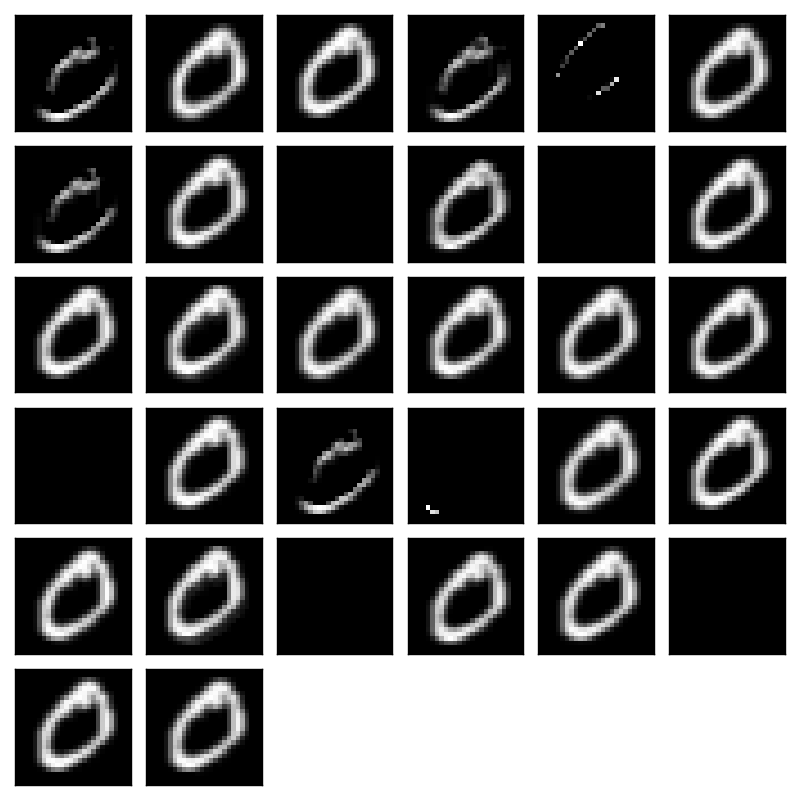
\includegraphics[height=4cm]{images/resultados/network_1/input_1_layer_activation_2}%
				\caption{Ativação}			
			\end{figure}%
		\end{column}	
	\end{columns}
	
\end{frame}
%%%%%%%%%%%%%%%%%%%%%%%%%%%%%%%%%%%%%%%%%%%%%%%%%%%%%%%%%%%%%%%%%%%%%%%%%%%%%%%%%%%%%%%%%%%

%%%%%%%%%%%%%%%%%%%%%%%%%%%%%%%%%%%%%%%%%%%%%%%%%%%%%%%%%%%%%%%%%%%%%%%%%%%%%%%%%%%%%%%%%%%
\begin{frame}
	\frametitle{Convolução - 3}
	\centering
	\begin{columns}
		\begin{column}{0.25\textwidth}
			\begin{figure}
				\resizebox{!}{.9\textheight}
				{% if required
					
					\begin{tikzpicture}[
					start chain=going below,
					every join/.style={arrow},
					node distance=0.3cm
					]
					\node (start) [startstop,on chain,join] {Imagem de entrada};
					
					\node (out1) [process3,on chain,join] {Convolução \\ Ativação};
					
					\node (out3) [process3,on chain,join] {Convolução \\ Ativação };
					
					\node (out5) [process2,on chain,join] {Convolução \\ Ativação};
					
					\node (out7) [process,on chain,join] {Pooling};
					
					\node (out8) [process,on chain,join] {Convolução \\ Ativação};
					
					\node (out10) [process,on chain,join] {Flatten};
					\node (out11) [process,on chain,join] {Dense};
					
					\node (out12) [process,on chain,join] {Dropout};
					\node (out13) [process,on chain,join] {Ativação};	
					
					\node (out14) [process,on chain,join] {Dense};
					\node (out15) [process,on chain,join] {Dropout};
					
					\node (out16) [startstop,on chain,join] {Ativação};		
					
					\end{tikzpicture}
				} %resize		
			\end{figure}
			
		\end{column}		
		
		\begin{column}{0.33\textwidth}
			\begin{figure}
				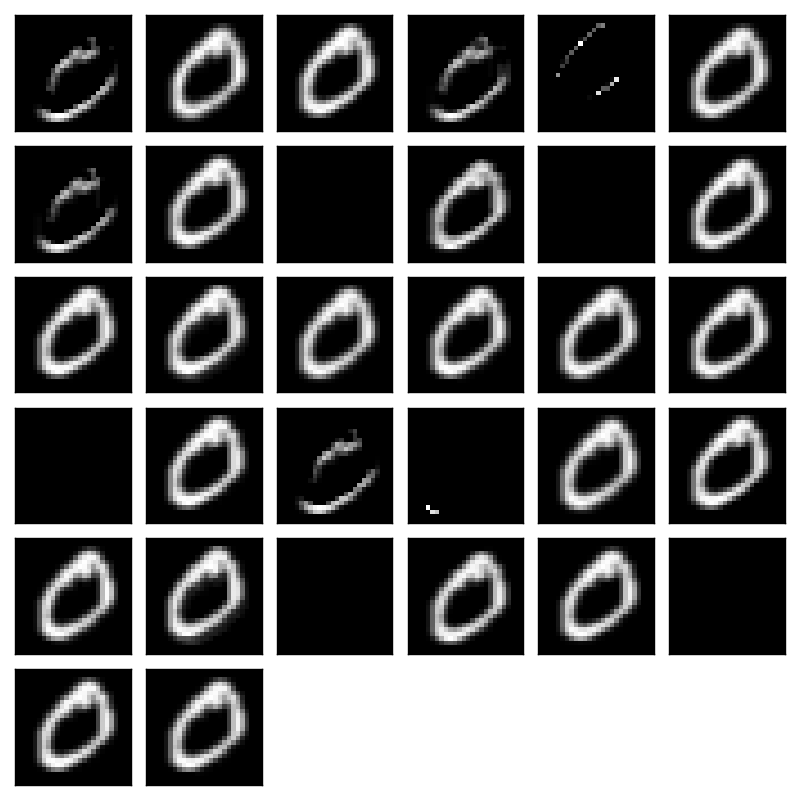
\includegraphics[height=4cm]{images/resultados/network_1/input_1_layer_activation_2}%
				\caption{Ativação 2}
			\end{figure}%
		\end{column}
		\begin{column}{0.33\textwidth}
			\begin{figure}
				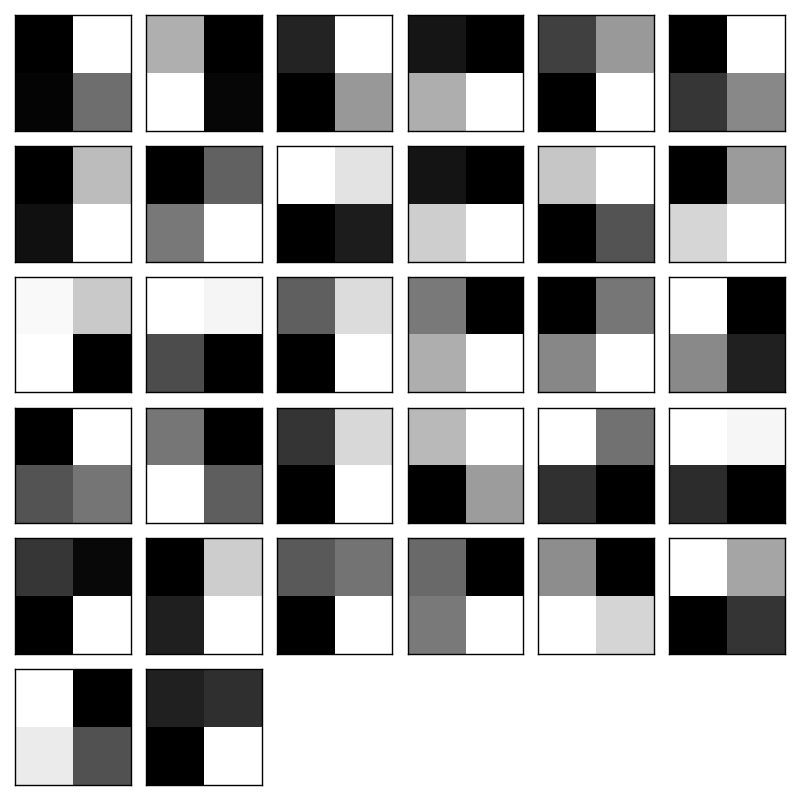
\includegraphics[height=4cm]{images/resultados/network_1/filter_convolution2d_3}%
				\caption{Filtros}			
			\end{figure}%
		\end{column}	
	\end{columns}
	
\end{frame}
%%%%%%%%%%%%%%%%%%%%%%%%%%%%%%%%%%%%%%%%%%%%%%%%%%%%%%%%%%%%%%%%%%%%%%%%%%%%%%%%%%%%%%%%%%%

%%%%%%%%%%%%%%%%%%%%%%%%%%%%%%%%%%%%%%%%%%%%%%%%%%%%%%%%%%%%%%%%%%%%%%%%%%%%%%%%%%%%%%%%%%%
\begin{frame}
	\frametitle{Convolução - 3}
	\centering
	\begin{columns}
		\begin{column}{0.25\textwidth}
			\begin{figure}
				\resizebox{!}{.9\textheight}
				{% if required
					
					\begin{tikzpicture}[
					start chain=going below,
					every join/.style={arrow},
					node distance=0.3cm
					]
					\node (start) [startstop,on chain,join] {Imagem de entrada};
					
					\node (out1) [process3,on chain,join] {Convolução \\ Ativação};
					
					\node (out3) [process3,on chain,join] {Convolução \\ Ativação };
					
					\node (out5) [process2,on chain,join] {Convolução \\ Ativação};
					
					\node (out7) [process,on chain,join] {Pooling};
					
					\node (out8) [process,on chain,join] {Convolução \\ Ativação};
					
					\node (out10) [process,on chain,join] {Flatten};
					\node (out11) [process,on chain,join] {Dense};
					
					\node (out12) [process,on chain,join] {Dropout};
					\node (out13) [process,on chain,join] {Ativação};	
					
					\node (out14) [process,on chain,join] {Dense};
					\node (out15) [process,on chain,join] {Dropout};
					
					\node (out16) [startstop,on chain,join] {Ativação};		
					
					\end{tikzpicture}
				} %resize		
			\end{figure}
			
		\end{column}		
		
		\begin{column}{0.33\textwidth}
			\begin{figure}
				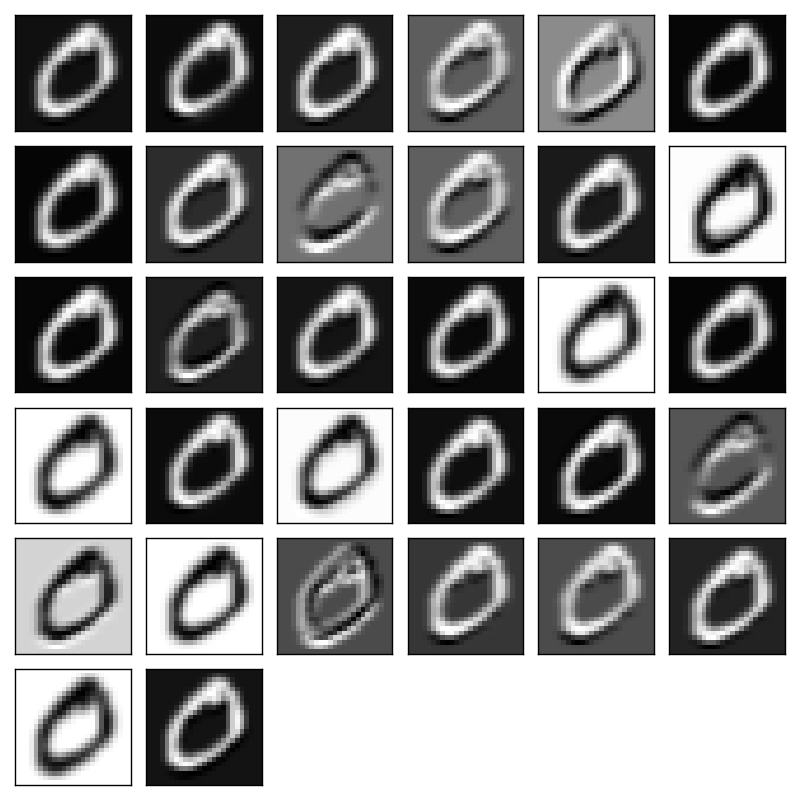
\includegraphics[height=4cm]{images/resultados/network_1/input_1_layer_convolution2d_3}%
				\caption{Convolução 3}
			\end{figure}%
		\end{column}
		\begin{column}{0.33\textwidth}
			\begin{figure}
				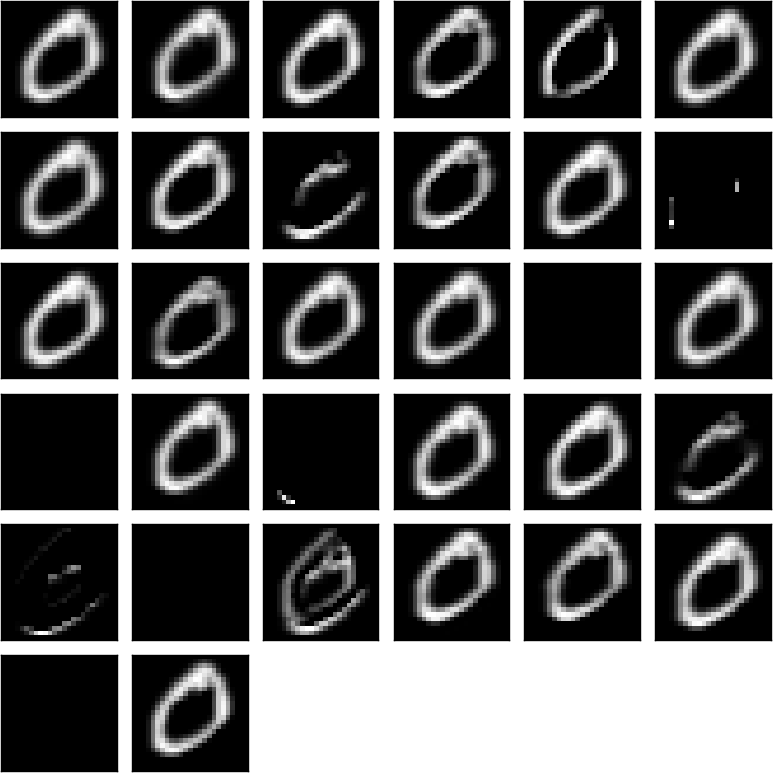
\includegraphics[height=4cm]{images/resultados/network_1/input_1_layer_activation_3}%
				\caption{Ativação}			
			\end{figure}%
		\end{column}	
	\end{columns}
	
\end{frame}
%%%%%%%%%%%%%%%%%%%%%%%%%%%%%%%%%%%%%%%%%%%%%%%%%%%%%%%%%%%%%%%%%%%%%%%%%%%%%%%%%%%%%%%%%%%


%%%%%%%%%%%%%%%%%%%%%%%%%%%%%%%%%%%%%%%%%%%%%%%%%%%%%%%%%%%%%%%%%%%%%%%%%%%%%%%%%%%%%%%%%%%
\begin{frame}
	\frametitle{Pooling - 1}
	\centering
	\begin{columns}
		\begin{column}{0.25\textwidth}
			\begin{figure}
				\resizebox{!}{.9\textheight}
				{% if required
					
					\begin{tikzpicture}[
					start chain=going below,
					every join/.style={arrow},
					node distance=0.3cm
					]
					\node (start) [startstop,on chain,join] {Imagem de entrada};
					
					\node (out1) [process3,on chain,join] {Convolução \\ Ativação};
					
					\node (out3) [process3,on chain,join] {Convolução \\ Ativação };
					
					\node (out5) [process3,on chain,join] {Convolução \\ Ativação};
					
					\node (out7) [process2,on chain,join] {Pooling};
					
					\node (out8) [process,on chain,join] {Convolução \\ Ativação};
					
					\node (out10) [process,on chain,join] {Flatten};
					\node (out11) [process,on chain,join] {Dense};
					
					\node (out12) [process,on chain,join] {Dropout};
					\node (out13) [process,on chain,join] {Ativação};	
					
					\node (out14) [process,on chain,join] {Dense};
					\node (out15) [process,on chain,join] {Dropout};
					
					\node (out16) [startstop,on chain,join] {Ativação};		
					
					\end{tikzpicture}
				} %resize		
			\end{figure}
			
		\end{column}		
		
		\begin{column}{0.33\textwidth}
			\begin{figure}
				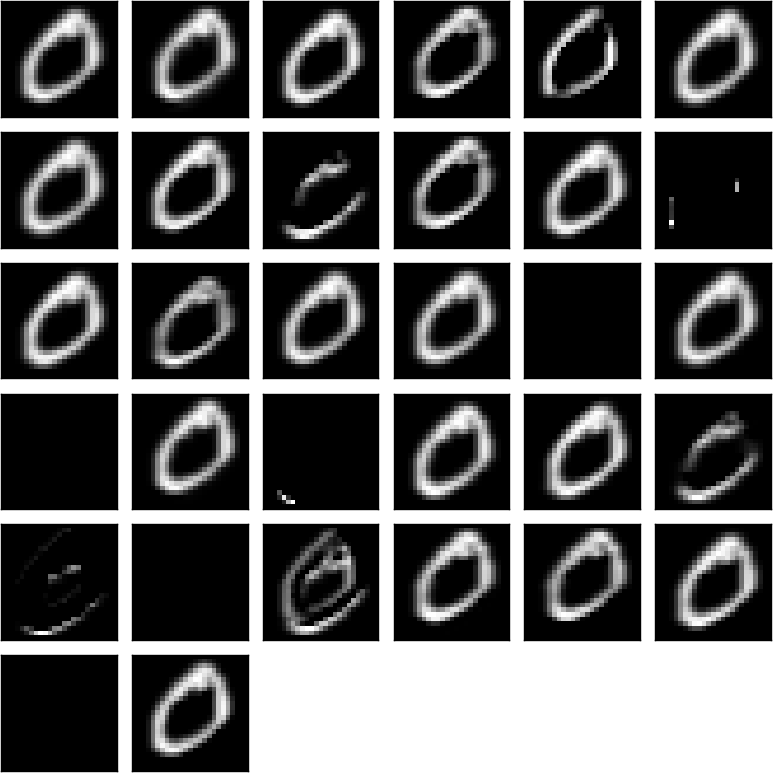
\includegraphics[height=4cm]{images/resultados/network_1/input_1_layer_activation_3}
				\caption{Ativação 3}
			\end{figure}%
		\end{column}
		\begin{column}{0.33\textwidth}
			\begin{figure}
				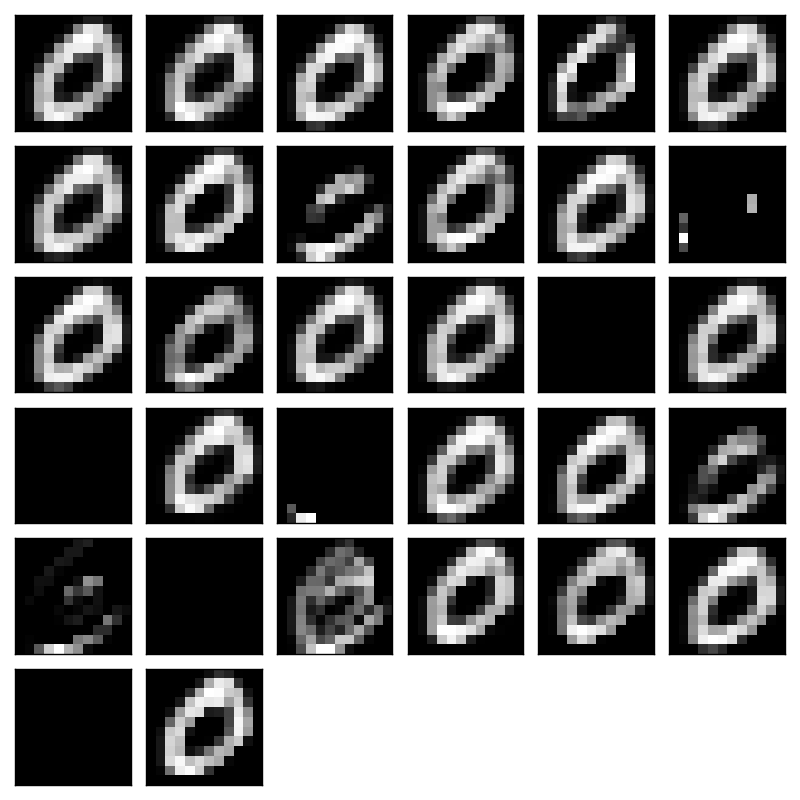
\includegraphics[height=4cm]{images/resultados/network_1/input_1_layer_maxpooling2d_1}%
				\caption{Pooling}			
			\end{figure}%
		\end{column}	
	\end{columns}
	
\end{frame}
%%%%%%%%%%%%%%%%%%%%%%%%%%%%%%%%%%%%%%%%%%%%%%%%%%%%%%%%%%%%%%%%%%%%%%%%%%%%%%%%%%%%%%%%%%%

%%%%%%%%%%%%%%%%%%%%%%%%%%%%%%%%%%%%%%%%%%%%%%%%%%%%%%%%%%%%%%%%%%%%%%%%%%%%%%%%%%%%%%%%%%%
\begin{frame}
	\frametitle{Convolução - 4}
	\centering
	\begin{columns}
		\begin{column}{0.25\textwidth}
			\begin{figure}
				\resizebox{!}{.9\textheight}
				{% if required
					
					\begin{tikzpicture}[
					start chain=going below,
					every join/.style={arrow},
					node distance=0.3cm
					]
					\node (start) [startstop,on chain,join] {Imagem de entrada};
					
					\node (out1) [process3,on chain,join] {Convolução \\ Ativação};
					
					\node (out3) [process3,on chain,join] {Convolução \\ Ativação };
					
					\node (out5) [process3,on chain,join] {Convolução \\ Ativação};
					
					\node (out7) [process3,on chain,join] {Pooling};
					
					\node (out8) [process2,on chain,join] {Convolução \\ Ativação};
					
					\node (out10) [process,on chain,join] {Flatten};
					\node (out11) [process,on chain,join] {Dense};
					
					\node (out12) [process,on chain,join] {Dropout};
					\node (out13) [process,on chain,join] {Ativação};	
					
					\node (out14) [process,on chain,join] {Dense};
					\node (out15) [process,on chain,join] {Dropout};
					
					\node (out16) [startstop,on chain,join] {Ativação};		
					
					\end{tikzpicture}
				} %resize		
			\end{figure}
			
		\end{column}		
		
		\begin{column}{0.33\textwidth}
			\begin{figure}
				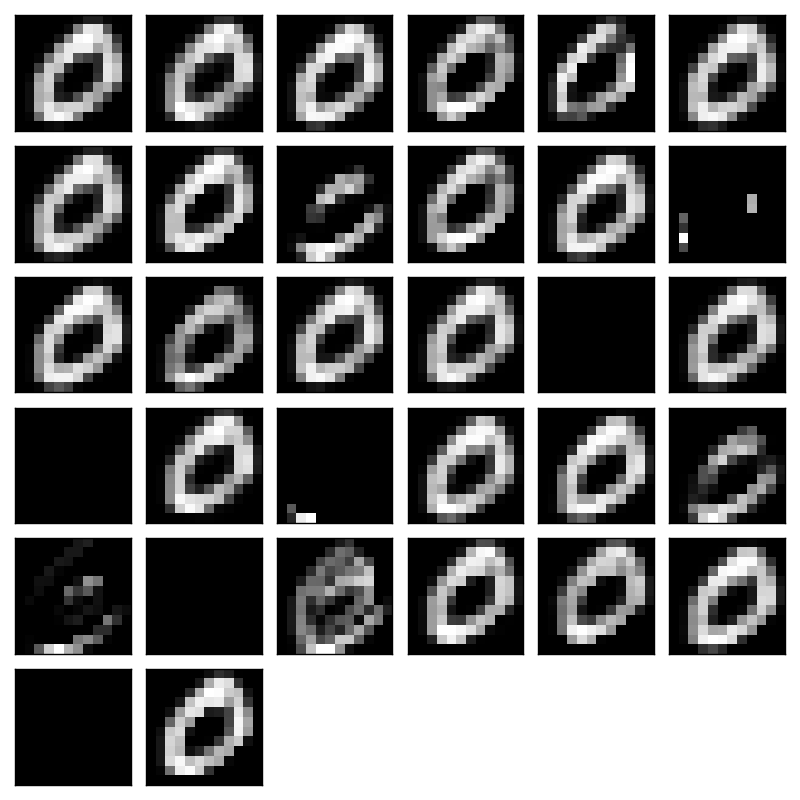
\includegraphics[height=4cm]{images/resultados/network_1/input_1_layer_maxpooling2d_1}
				\caption{Pooling 1}
			\end{figure}%
		\end{column}
		\begin{column}{0.33\textwidth}
			\begin{figure}
				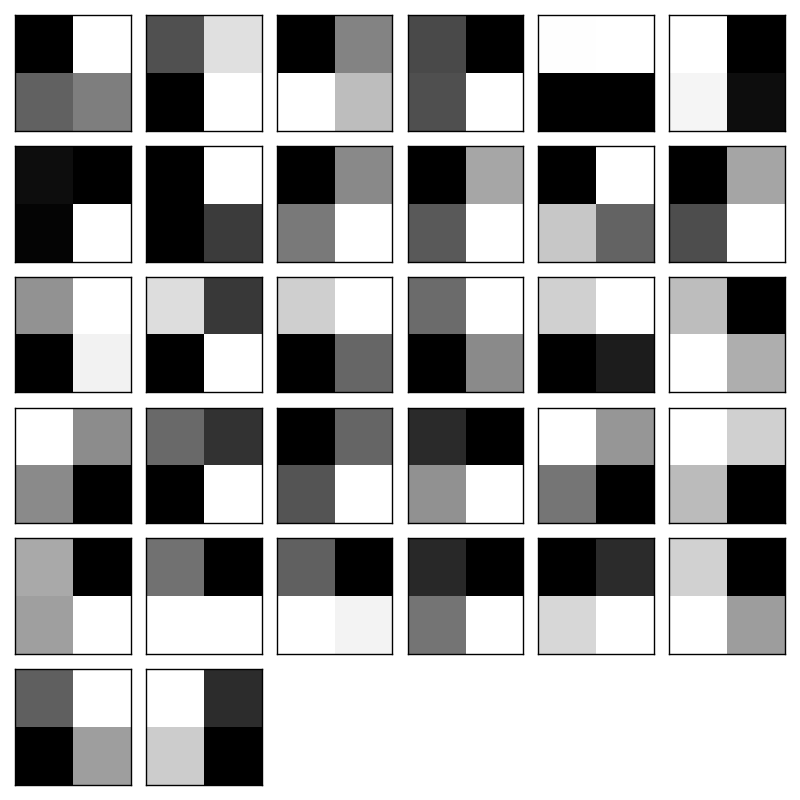
\includegraphics[height=4cm]{images/resultados/network_1/filter_convolution2d_4}%
				\caption{Filtros}			
			\end{figure}%
		\end{column}	
	\end{columns}
	
\end{frame}
%%%%%%%%%%%%%%%%%%%%%%%%%%%%%%%%%%%%%%%%%%%%%%%%%%%%%%%%%%%%%%%%%%%%%%%%%%%%%%%%%%%%%%%%%%%

%%%%%%%%%%%%%%%%%%%%%%%%%%%%%%%%%%%%%%%%%%%%%%%%%%%%%%%%%%%%%%%%%%%%%%%%%%%%%%%%%%%%%%%%%%%
\begin{frame}
	\frametitle{Convolução - 4}
	\centering
	\begin{columns}
		\begin{column}{0.25\textwidth}
			\begin{figure}
				\resizebox{!}{.9\textheight}
				{% if required
					
					\begin{tikzpicture}[
					start chain=going below,
					every join/.style={arrow},
					node distance=0.3cm
					]
					\node (start) [startstop,on chain,join] {Imagem de entrada};
					
					\node (out1) [process3,on chain,join] {Convolução \\ Ativação};
					
					\node (out3) [process3,on chain,join] {Convolução \\ Ativação };
					
					\node (out5) [process3,on chain,join] {Convolução \\ Ativação};
					
					\node (out7) [process3,on chain,join] {Pooling};
					
					\node (out8) [process2,on chain,join] {Convolução \\ Ativação};
					
					\node (out10) [process,on chain,join] {Flatten};
					\node (out11) [process,on chain,join] {Dense};
					
					\node (out12) [process,on chain,join] {Dropout};
					\node (out13) [process,on chain,join] {Ativação};	
					
					\node (out14) [process,on chain,join] {Dense};
					\node (out15) [process,on chain,join] {Dropout};
					
					\node (out16) [startstop,on chain,join] {Ativação};		
					
					\end{tikzpicture}
				} %resize		
			\end{figure}
			
		\end{column}		
		
		\begin{column}{0.33\textwidth}
			\begin{figure}
				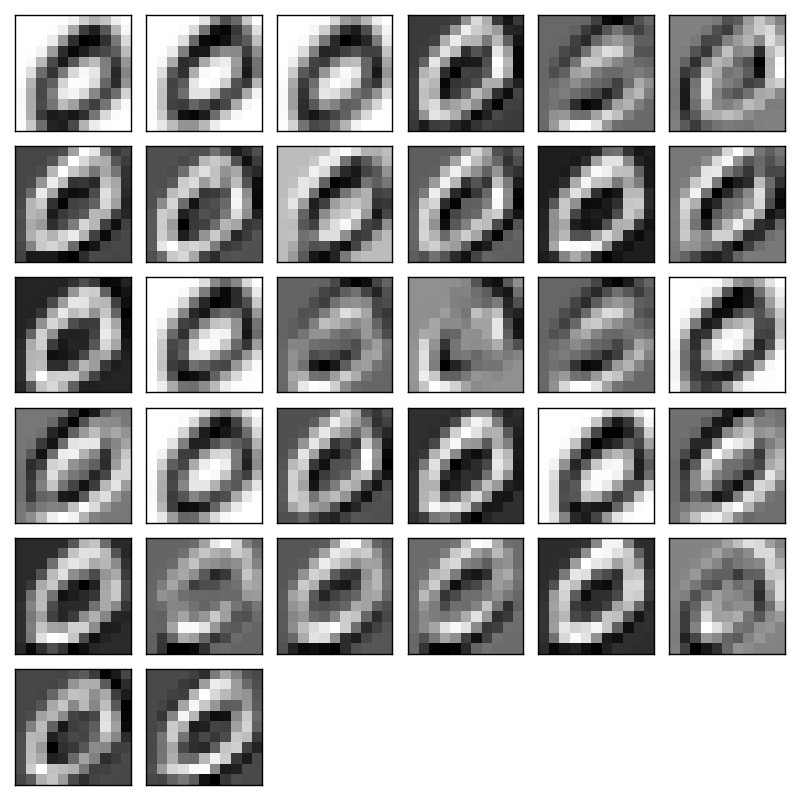
\includegraphics[height=4cm]{images/resultados/network_1/input_1_layer_convolution2d_4}
				\caption{Convolução 4}
			\end{figure}%
		\end{column}
		\begin{column}{0.33\textwidth}
			\begin{figure}
				
\includegraphics[height=4cm]{images/resultados/network_1/input_1_layer_activation_4}%
				\caption{Ativação}			
			\end{figure}%
		\end{column}	
	\end{columns}
	
\end{frame}
%%%%%%%%%%%%%%%%%%%%%%%%%%%%%%%%%%%%%%%%%%%%%%%%%%%%%%%%%%%%%%%%%%%%%%%%%%%%%%%%%%%%%%%%%%%

%%%%%%%%%%%%%%%%%%%%%%%%%%%%%%%%%%%%%%%%%%%%%%%%%%%%%%%%%%%%%%%%%%%%%%%%%%%%%%%%%%%%%%%%%%%
\begin{frame}
	\frametitle{Flatten}
	\centering
	\begin{columns}
		\begin{column}{0.25\textwidth}
			\begin{figure}
				\resizebox{!}{.9\textheight}
				{% if required
					
					\begin{tikzpicture}[
					start chain=going below,
					every join/.style={arrow},
					node distance=0.3cm
					]
					\node (start) [startstop,on chain,join] {Imagem de entrada};
					
					\node (out1) [process3,on chain,join] {Convolução \\ Ativação};
					
					\node (out3) [process3,on chain,join] {Convolução \\ Ativação };
					
					\node (out5) [process3,on chain,join] {Convolução \\ Ativação};
					
					\node (out7) [process3,on chain,join] {Pooling};
					
					\node (out8) [process3,on chain,join] {Convolução \\ Ativação};
					
					\node (out10) [process2,on chain,join] {Flatten};
					\node (out11) [process,on chain,join] {Dense};
					
					\node (out12) [process,on chain,join] {Dropout};
					\node (out13) [process,on chain,join] {Ativação};	
					
					\node (out14) [process,on chain,join] {Dense};
					\node (out15) [process,on chain,join] {Dropout};
					
					\node (out16) [startstop,on chain,join] {Ativação};		
					
					\end{tikzpicture}
				} %resize		
			\end{figure}
			
		\end{column}		
		
		\begin{column}{0.66\textwidth}
			\begin{figure}
				
\includegraphics[height=4cm]{images/resultados/network_1/input_1_layer_activation_4}
				\caption{Ativação 4}
			\end{figure}%
			\begin{figure}
				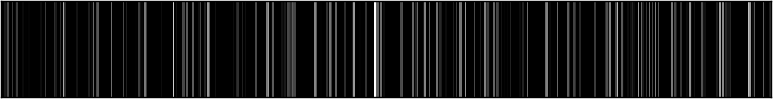
\includegraphics[width=6cm]{images/resultados/network_1/input_1_layer_flatten_1}%
				\caption{Flatten \small{ ( $3 \times 3 \times 32 \rightarrow 1 \times 1 \times 288$ )} }			
			\end{figure}%
		\end{column}	
	\end{columns}
	
\end{frame}
%%%%%%%%%%%%%%%%%%%%%%%%%%%%%%%%%%%%%%%%%%%%%%%%%%%%%%%%%%%%%%%%%%%%%%%%%%%%%%%%%%%%%%%%%%%

%%%%%%%%%%%%%%%%%%%%%%%%%%%%%%%%%%%%%%%%%%%%%%%%%%%%%%%%%%%%%%%%%%%%%%%%%%%%%%%%%%%%%%%%%%%
\begin{frame}
	\frametitle{Dense - 1}
	\centering
	\begin{columns}
		\begin{column}{0.25\textwidth}
			\begin{figure}
				\resizebox{!}{.9\textheight}
				{% if required
					
					\begin{tikzpicture}[
					start chain=going below,
					every join/.style={arrow},
					node distance=0.3cm
					]
					\node (start) [startstop,on chain,join] {Imagem de entrada};
					
					\node (out1) [process3,on chain,join] {Convolução \\ Ativação};
					
					\node (out3) [process3,on chain,join] {Convolução \\ Ativação };
					
					\node (out5) [process3,on chain,join] {Convolução \\ Ativação};
					
					\node (out7) [process3,on chain,join] {Pooling};
					
					\node (out8) [process3,on chain,join] {Convolução \\ Ativação};
					
					\node (out10) [process3,on chain,join] {Flatten};
					\node (out11) [process2,on chain,join] {Dense};
					
					\node (out12) [process,on chain,join] {Dropout};
					\node (out13) [process,on chain,join] {Ativação};	
					
					\node (out14) [process,on chain,join] {Dense};
					\node (out15) [process,on chain,join] {Dropout};
					
					\node (out16) [startstop,on chain,join] {Ativação};		
					
					\end{tikzpicture}
				} %resize		
			\end{figure}
			
		\end{column}		
		
		\begin{column}{0.66\textwidth}
			\begin{figure}
				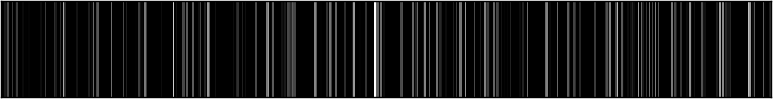
\includegraphics[width=6cm]{images/resultados/network_1/input_1_layer_flatten_1}%
				\caption{Flatten \small{1x1x288} }	
			\end{figure}%
			\begin{figure}
				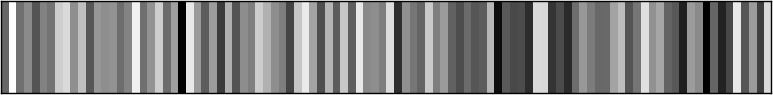
\includegraphics[width=6cm]{images/resultados/network_1/input_1_layer_dense_1}%
				\caption{Dense \small{1x1x100} }			
			\end{figure}%
		\end{column}	
	\end{columns}
	
\end{frame}
%%%%%%%%%%%%%%%%%%%%%%%%%%%%%%%%%%%%%%%%%%%%%%%%%%%%%%%%%%%%%%%%%%%%%%%%%%%%%%%%%%%%%%%%%%%

%%%%%%%%%%%%%%%%%%%%%%%%%%%%%%%%%%%%%%%%%%%%%%%%%%%%%%%%%%%%%%%%%%%%%%%%%%%%%%%%%%%%%%%%%%%
\begin{frame}
	\frametitle{Dropout - 1}
	\centering
	\begin{columns}
		\begin{column}{0.25\textwidth}
			\begin{figure}
				\resizebox{!}{.9\textheight}
				{% if required
					
					\begin{tikzpicture}[
					start chain=going below,
					every join/.style={arrow},
					node distance=0.3cm
					]
					\node (start) [startstop,on chain,join] {Imagem de entrada};
					
					\node (out1) [process3,on chain,join] {Convolução \\ Ativação};
					
					\node (out3) [process3,on chain,join] {Convolução \\ Ativação };
					
					\node (out5) [process3,on chain,join] {Convolução \\ Ativação};
					
					\node (out7) [process3,on chain,join] {Pooling};
					
					\node (out8) [process3,on chain,join] {Convolução \\ Ativação};
					
					\node (out10) [process3,on chain,join] {Flatten};
					\node (out11) [process3,on chain,join] {Dense};
					
					\node (out12) [process2,on chain,join] {Dropout};
					\node (out13) [process,on chain,join] {Ativação};	
					
					\node (out14) [process,on chain,join] {Dense};
					\node (out15) [process,on chain,join] {Dropout};
					
					\node (out16) [startstop,on chain,join] {Ativação};		
					
					\end{tikzpicture}
				} %resize		
			\end{figure}
			
		\end{column}		
		
		\begin{column}{0.66\textwidth}
			\begin{itemize}
				\item Dropout = 0.25
			\end{itemize}			
		\end{column}	
	\end{columns}
	
\end{frame}
%%%%%%%%%%%%%%%%%%%%%%%%%%%%%%%%%%%%%%%%%%%%%%%%%%%%%%%%%%%%%%%%%%%%%%%%%%%%%%%%%%%%%%%%%%%

%%%%%%%%%%%%%%%%%%%%%%%%%%%%%%%%%%%%%%%%%%%%%%%%%%%%%%%%%%%%%%%%%%%%%%%%%%%%%%%%%%%%%%%%%%%
\begin{frame}
	\frametitle{Ativação - 7}
	\centering
	\begin{columns}
		\begin{column}{0.25\textwidth}
			\begin{figure}
				\resizebox{!}{.9\textheight}
				{% if required
					
					\begin{tikzpicture}[
					start chain=going below,
					every join/.style={arrow},
					node distance=0.3cm
					]
					\node (start) [startstop,on chain,join] {Imagem de entrada};
					
					\node (out1) [process3,on chain,join] {Convolução \\ Ativação};
					
					\node (out3) [process3,on chain,join] {Convolução \\ Ativação };
					
					\node (out5) [process3,on chain,join] {Convolução \\ Ativação};
					
					\node (out7) [process3,on chain,join] {Pooling};
					
					\node (out8) [process3,on chain,join] {Convolução \\ Ativação};
					
					\node (out10) [process3,on chain,join] {Flatten};
					\node (out11) [process3,on chain,join] {Dense};
					
					\node (out12) [process3,on chain,join] {Dropout};
					\node (out13) [process2,on chain,join] {Ativação};	
					
					\node (out14) [process,on chain,join] {Dense};
					\node (out15) [process,on chain,join] {Dropout};
					
					\node (out16) [startstop,on chain,join] {Ativação};		
					
					\end{tikzpicture}
				} %resize		
			\end{figure}
			
		\end{column}		
		
		\begin{column}{0.66\textwidth}
			\begin{figure}
				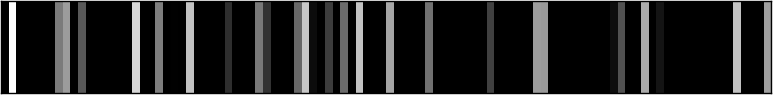
\includegraphics[width=6cm]{images/resultados/network_1/input_1_layer_activation_7}%
				\caption{Ativação }			
			\end{figure}%
		\end{column}	
	\end{columns}
	
\end{frame}
%%%%%%%%%%%%%%%%%%%%%%%%%%%%%%%%%%%%%%%%%%%%%%%%%%%%%%%%%%%%%%%%%%%%%%%%%%%%%%%%%%%%%%%%%%%

%%%%%%%%%%%%%%%%%%%%%%%%%%%%%%%%%%%%%%%%%%%%%%%%%%%%%%%%%%%%%%%%%%%%%%%%%%%%%%%%%%%%%%%%%%%
\begin{frame}
	\frametitle{Dense - 2}
	\centering
	\begin{columns}
		\begin{column}{0.25\textwidth}
			\begin{figure}
				\resizebox{!}{.9\textheight}
				{% if required
					
					\begin{tikzpicture}[
					start chain=going below,
					every join/.style={arrow},
					node distance=0.3cm
					]
					\node (start) [startstop,on chain,join] {Imagem de entrada};
					
					\node (out1) [process3,on chain,join] {Convolução \\ Ativação};
					
					\node (out3) [process3,on chain,join] {Convolução \\ Ativação };
					
					\node (out5) [process3,on chain,join] {Convolução \\ Ativação};
					
					\node (out7) [process3,on chain,join] {Pooling};
					
					\node (out8) [process3,on chain,join] {Convolução \\ Ativação};
					
					\node (out10) [process3,on chain,join] {Flatten};
					\node (out11) [process3,on chain,join] {Dense};
					
					\node (out12) [process3,on chain,join] {Dropout};
					\node (out13) [process3,on chain,join] {Ativação};	
					
					\node (out14) [process2,on chain,join] {Dense};
					\node (out15) [process,on chain,join] {Dropout};
					
					\node (out16) [startstop,on chain,join] {Ativação};		
					
					\end{tikzpicture}
				} %resize		
			\end{figure}
			
		\end{column}		
		
		\begin{column}{0.66\textwidth}
			\begin{figure}
				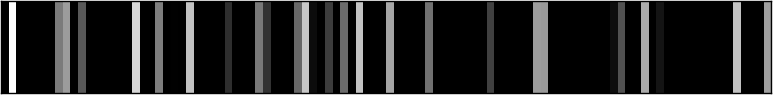
\includegraphics[width=6cm]{images/resultados/network_1/input_1_layer_activation_7}%
				\caption{Ativação 7 \small{1x1x100} }	
			\end{figure}%
			\begin{figure}
				
\includegraphics[width=6cm]{images/resultados/network_1/input_1_layer_dense_2}%
				\caption{Dense \small{1x1x10} }			
			\end{figure}%
		\end{column}	
	\end{columns}
	
\end{frame}
%%%%%%%%%%%%%%%%%%%%%%%%%%%%%%%%%%%%%%%%%%%%%%%%%%%%%%%%%%%%%%%%%%%%%%%%%%%%%%%%%%%%%%%%%%%

%%%%%%%%%%%%%%%%%%%%%%%%%%%%%%%%%%%%%%%%%%%%%%%%%%%%%%%%%%%%%%%%%%%%%%%%%%%%%%%%%%%%%%%%%%%
\begin{frame}
	\frametitle{Dropout - 2}
	\centering
	\begin{columns}
		\begin{column}{0.25\textwidth}
			\begin{figure}
				\resizebox{!}{.9\textheight}
				{% if required
					
					\begin{tikzpicture}[
					start chain=going below,
					every join/.style={arrow},
					node distance=0.3cm
					]
					\node (start) [startstop,on chain,join] {Imagem de entrada};
					
					\node (out1) [process3,on chain,join] {Convolução \\ Ativação};
					
					\node (out3) [process3,on chain,join] {Convolução \\ Ativação };
					
					\node (out5) [process3,on chain,join] {Convolução \\ Ativação};
					
					\node (out7) [process3,on chain,join] {Pooling};
					
					\node (out8) [process3,on chain,join] {Convolução \\ Ativação};
					
					\node (out10) [process3,on chain,join] {Flatten};
					\node (out11) [process3,on chain,join] {Dense};
					
					\node (out12) [process3,on chain,join] {Dropout};
					\node (out13) [process3,on chain,join] {Ativação};	
					
					\node (out14) [process3,on chain,join] {Dense};
					\node (out15) [process2,on chain,join] {Dropout};
					
					\node (out16) [startstop,on chain,join] {Ativação};		
					
					\end{tikzpicture}
				} %resize		
			\end{figure}
			
		\end{column}		
		
		\begin{column}{0.66\textwidth}
			\begin{itemize}
				\item Dropout = 0.25
			\end{itemize}			
		\end{column}	
	\end{columns}
	
\end{frame}
%%%%%%%%%%%%%%%%%%%%%%%%%%%%%%%%%%%%%%%%%%%%%%%%%%%%%%%%%%%%%%%%%%%%%%%%%%%%%%%%%%%%%%%%%%%

%%%%%%%%%%%%%%%%%%%%%%%%%%%%%%%%%%%%%%%%%%%%%%%%%%%%%%%%%%%%%%%%%%%%%%%%%%%%%%%%%%%%%%%%%%%
\begin{frame}
	\frametitle{Ativação - 8}
	\centering
	\begin{columns}
		\begin{column}{0.25\textwidth}
			\begin{figure}
				\resizebox{!}{.9\textheight}
				{% if required
					
					\begin{tikzpicture}[
					start chain=going below,
					every join/.style={arrow},
					node distance=0.3cm
					]
					\node (start) [startstop,on chain,join] {Imagem de entrada};
					
					\node (out1) [process3,on chain,join] {Convolução \\ Ativação};
					
					\node (out3) [process3,on chain,join] {Convolução \\ Ativação };
					
					\node (out5) [process3,on chain,join] {Convolução \\ Ativação};
					
					\node (out7) [process3,on chain,join] {Pooling};
					
					\node (out8) [process3,on chain,join] {Convolução \\ Ativação};
					
					\node (out10) [process3,on chain,join] {Flatten};
					\node (out11) [process3,on chain,join] {Dense};
					
					\node (out12) [process3,on chain,join] {Dropout};
					\node (out13) [process3,on chain,join] {Ativação};	
					
					\node (out14) [process3,on chain,join] {Dense};
					\node (out15) [process3,on chain,join] {Dropout};
					
					\node (out16) [startstop,on chain,join] {Ativação};		
					
					\end{tikzpicture}
				} %resize		
			\end{figure}
			
		\end{column}		
		
		\begin{column}{0.66\textwidth}
			\begin{figure}
				
\includegraphics[width=6cm]{images/resultados/network_1/input_1_layer_activation_8}%
				\caption{Ativação }			
			\end{figure}%
		\end{column}	
	\end{columns}
	
\end{frame}
%%%%%%%%%%%%%%%%%%%%%%%%%%%%%%%%%%%%%%%%%%%%%%%%%%%%%%%%%%%%%%%%%%%%%%%%%%%%%%%%%%%%%%%%%%%

\begin{frame}
	\frametitle{Outros exemplos de redes convolucionais}
	\begin{itemize}
		\item CNNs podem ser utilizadas para entradas bidimensionais como por exemplo reconhecimento de voz.
		\item \textit{Convolutional Neural Networks for Speech Recognition (Ossama A.H. et Al., 2014 - Microsoft)}
	\end{itemize}
	\begin{center}
		\begin{figure}
		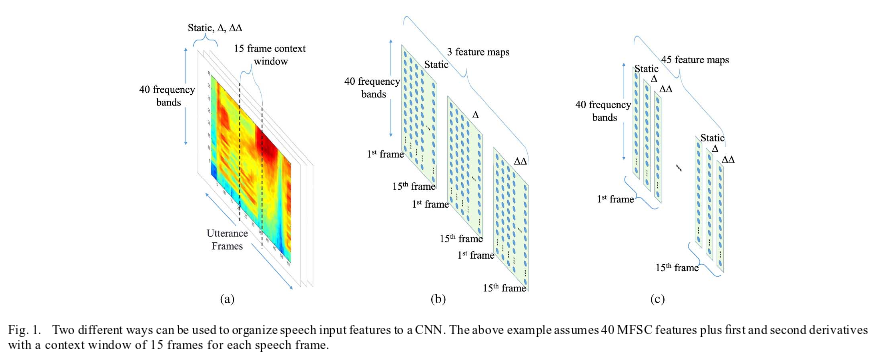
\includegraphics[width=0.9\textwidth]{images/fabio/ossama_et_al}
		\caption{Imagem de Ossama A.H. et Al., 2014 exemplificado entrada e processamento no reconhecimento de voz com redes neurais convolucionais}
		\end{figure}
	\end{center}

\end{frame}

\begin{frame}
	\frametitle{MLP \& CNN}
	\centering
	\begin{itemize}
		\item CNN é uma extensão do conceito da MLP
		\item Convoluções e Pooling ajudam a diminuir rapidamente o número de variáveis do sistema
		\item Próprio para o processamento de imagens e vídeos		
	\end{itemize}
\end{frame}

% -------------------------------------------------
% end{fabio}
% -------------------------------------------------
\end{document}